\PassOptionsToPackage{unicode=true}{hyperref} % options for packages loaded elsewhere
\PassOptionsToPackage{hyphens}{url}
%
\documentclass[
]{book}
\usepackage{lmodern}
\usepackage{amssymb,amsmath}
\usepackage{ifxetex,ifluatex}
\ifnum 0\ifxetex 1\fi\ifluatex 1\fi=0 % if pdftex
  \usepackage[T1]{fontenc}
  \usepackage[utf8]{inputenc}
  \usepackage{textcomp} % provides euro and other symbols
\else % if luatex or xelatex
  \usepackage{unicode-math}
  \defaultfontfeatures{Scale=MatchLowercase}
  \defaultfontfeatures[\rmfamily]{Ligatures=TeX,Scale=1}
\fi
% use upquote if available, for straight quotes in verbatim environments
\IfFileExists{upquote.sty}{\usepackage{upquote}}{}
\IfFileExists{microtype.sty}{% use microtype if available
  \usepackage[]{microtype}
  \UseMicrotypeSet[protrusion]{basicmath} % disable protrusion for tt fonts
}{}
\makeatletter
\@ifundefined{KOMAClassName}{% if non-KOMA class
  \IfFileExists{parskip.sty}{%
    \usepackage{parskip}
  }{% else
    \setlength{\parindent}{0pt}
    \setlength{\parskip}{6pt plus 2pt minus 1pt}}
}{% if KOMA class
  \KOMAoptions{parskip=half}}
\makeatother
\usepackage{xcolor}
\IfFileExists{xurl.sty}{\usepackage{xurl}}{} % add URL line breaks if available
\IfFileExists{bookmark.sty}{\usepackage{bookmark}}{\usepackage{hyperref}}
\hypersetup{
  pdftitle={Modelos Estadísticos},
  pdfauthor={Javier Morales (Universidad Miguel Hernández de Elche); Mª Asunción Martínez (Universidad Miguel Hernández de Elche)},
  pdfborder={0 0 0},
  breaklinks=true}
\urlstyle{same}  % don't use monospace font for urls
\usepackage{color}
\usepackage{fancyvrb}
\newcommand{\VerbBar}{|}
\newcommand{\VERB}{\Verb[commandchars=\\\{\}]}
\DefineVerbatimEnvironment{Highlighting}{Verbatim}{commandchars=\\\{\}}
% Add ',fontsize=\small' for more characters per line
\usepackage{framed}
\definecolor{shadecolor}{RGB}{248,248,248}
\newenvironment{Shaded}{\begin{snugshade}}{\end{snugshade}}
\newcommand{\AlertTok}[1]{\textcolor[rgb]{0.94,0.16,0.16}{#1}}
\newcommand{\AnnotationTok}[1]{\textcolor[rgb]{0.56,0.35,0.01}{\textbf{\textit{#1}}}}
\newcommand{\AttributeTok}[1]{\textcolor[rgb]{0.77,0.63,0.00}{#1}}
\newcommand{\BaseNTok}[1]{\textcolor[rgb]{0.00,0.00,0.81}{#1}}
\newcommand{\BuiltInTok}[1]{#1}
\newcommand{\CharTok}[1]{\textcolor[rgb]{0.31,0.60,0.02}{#1}}
\newcommand{\CommentTok}[1]{\textcolor[rgb]{0.56,0.35,0.01}{\textit{#1}}}
\newcommand{\CommentVarTok}[1]{\textcolor[rgb]{0.56,0.35,0.01}{\textbf{\textit{#1}}}}
\newcommand{\ConstantTok}[1]{\textcolor[rgb]{0.00,0.00,0.00}{#1}}
\newcommand{\ControlFlowTok}[1]{\textcolor[rgb]{0.13,0.29,0.53}{\textbf{#1}}}
\newcommand{\DataTypeTok}[1]{\textcolor[rgb]{0.13,0.29,0.53}{#1}}
\newcommand{\DecValTok}[1]{\textcolor[rgb]{0.00,0.00,0.81}{#1}}
\newcommand{\DocumentationTok}[1]{\textcolor[rgb]{0.56,0.35,0.01}{\textbf{\textit{#1}}}}
\newcommand{\ErrorTok}[1]{\textcolor[rgb]{0.64,0.00,0.00}{\textbf{#1}}}
\newcommand{\ExtensionTok}[1]{#1}
\newcommand{\FloatTok}[1]{\textcolor[rgb]{0.00,0.00,0.81}{#1}}
\newcommand{\FunctionTok}[1]{\textcolor[rgb]{0.00,0.00,0.00}{#1}}
\newcommand{\ImportTok}[1]{#1}
\newcommand{\InformationTok}[1]{\textcolor[rgb]{0.56,0.35,0.01}{\textbf{\textit{#1}}}}
\newcommand{\KeywordTok}[1]{\textcolor[rgb]{0.13,0.29,0.53}{\textbf{#1}}}
\newcommand{\NormalTok}[1]{#1}
\newcommand{\OperatorTok}[1]{\textcolor[rgb]{0.81,0.36,0.00}{\textbf{#1}}}
\newcommand{\OtherTok}[1]{\textcolor[rgb]{0.56,0.35,0.01}{#1}}
\newcommand{\PreprocessorTok}[1]{\textcolor[rgb]{0.56,0.35,0.01}{\textit{#1}}}
\newcommand{\RegionMarkerTok}[1]{#1}
\newcommand{\SpecialCharTok}[1]{\textcolor[rgb]{0.00,0.00,0.00}{#1}}
\newcommand{\SpecialStringTok}[1]{\textcolor[rgb]{0.31,0.60,0.02}{#1}}
\newcommand{\StringTok}[1]{\textcolor[rgb]{0.31,0.60,0.02}{#1}}
\newcommand{\VariableTok}[1]{\textcolor[rgb]{0.00,0.00,0.00}{#1}}
\newcommand{\VerbatimStringTok}[1]{\textcolor[rgb]{0.31,0.60,0.02}{#1}}
\newcommand{\WarningTok}[1]{\textcolor[rgb]{0.56,0.35,0.01}{\textbf{\textit{#1}}}}
\usepackage{longtable,booktabs}
% Allow footnotes in longtable head/foot
\IfFileExists{footnotehyper.sty}{\usepackage{footnotehyper}}{\usepackage{footnote}}
\makesavenoteenv{longtable}
\usepackage{graphicx,grffile}
\makeatletter
\def\maxwidth{\ifdim\Gin@nat@width>\linewidth\linewidth\else\Gin@nat@width\fi}
\def\maxheight{\ifdim\Gin@nat@height>\textheight\textheight\else\Gin@nat@height\fi}
\makeatother
% Scale images if necessary, so that they will not overflow the page
% margins by default, and it is still possible to overwrite the defaults
% using explicit options in \includegraphics[width, height, ...]{}
\setkeys{Gin}{width=\maxwidth,height=\maxheight,keepaspectratio}
\setlength{\emergencystretch}{3em}  % prevent overfull lines
\providecommand{\tightlist}{%
  \setlength{\itemsep}{0pt}\setlength{\parskip}{0pt}}
\setcounter{secnumdepth}{5}
% Redefines (sub)paragraphs to behave more like sections
\ifx\paragraph\undefined\else
  \let\oldparagraph\paragraph
  \renewcommand{\paragraph}[1]{\oldparagraph{#1}\mbox{}}
\fi
\ifx\subparagraph\undefined\else
  \let\oldsubparagraph\subparagraph
  \renewcommand{\subparagraph}[1]{\oldsubparagraph{#1}\mbox{}}
\fi

% set default figure placement to htbp
\makeatletter
\def\fps@figure{htbp}
\makeatother

\usepackage{booktabs}
\usepackage[]{natbib}
\bibliographystyle{apalike}

\title{Modelos Estadísticos}
\author{Javier Morales (Universidad Miguel Hernández de Elche) \and Mª Asunción Martínez (Universidad Miguel Hernández de Elche)}
\date{2020-05-02}

\usepackage{amsthm}
\newtheorem{theorem}{Teorema}[chapter]
\newtheorem{lemma}{Lema}[chapter]
\newtheorem{corollary}{Corolario}[chapter]
\newtheorem{proposition}{Proposición}[chapter]
\newtheorem{conjecture}{Conjecture}[chapter]
\theoremstyle{definition}
\newtheorem{definition}{Definición}[chapter]
\theoremstyle{definition}
\newtheorem{example}{Ejemplo}[chapter]
\theoremstyle{definition}
\newtheorem{exercise}{Ejercicio}[chapter]
\theoremstyle{remark}
\newtheorem*{remark}{Nota: }
\newtheorem*{solution}{Solución}
\let\BeginKnitrBlock\begin \let\EndKnitrBlock\end
\begin{document}
\frontmatter
\maketitle

{
\setcounter{tocdepth}{1}
\tableofcontents
}
\mainmatter
\hypertarget{introducciuxf3n}{%
\chapter*{Introducción}\label{introducciuxf3n}}
\addcontentsline{toc}{chapter}{Introducción}

\begin{Shaded}
\begin{Highlighting}[]
\KeywordTok{library}\NormalTok{(tidyverse)}
\KeywordTok{library}\NormalTok{(tidymodels)}
\KeywordTok{library}\NormalTok{(stringr)}
\KeywordTok{library}\NormalTok{(forcats)}
\KeywordTok{library}\NormalTok{(lubridate)}
\KeywordTok{library}\NormalTok{(magrittr)}
\KeywordTok{library}\NormalTok{(broom)}
\KeywordTok{library}\NormalTok{(datasets)}
\KeywordTok{library}\NormalTok{(lmtest)}
\KeywordTok{library}\NormalTok{(MASS)}
\KeywordTok{library}\NormalTok{(kableExtra)}
\KeywordTok{library}\NormalTok{(mosaic)}
\KeywordTok{library}\NormalTok{(latex2exp)}
\KeywordTok{library}\NormalTok{(pubh)}
\KeywordTok{library}\NormalTok{(moonBook)}
\KeywordTok{library}\NormalTok{(sjlabelled)}
\KeywordTok{library}\NormalTok{(sjPlot)}
\KeywordTok{library}\NormalTok{(nasaweather)}
\KeywordTok{library}\NormalTok{(alr3)}
\KeywordTok{library}\NormalTok{(reshape2)}
\KeywordTok{library}\NormalTok{(olsrr)}
\KeywordTok{library}\NormalTok{(ggfortify)}
\KeywordTok{library}\NormalTok{(equatiomatic) }\CommentTok{# necesario solo para escritura markdown}
\end{Highlighting}
\end{Shaded}

Para instalar los paquetes necesarios para poder ejecutar la sintáxis mostrada en el libro se puede emplear el siguiente comando:

\begin{Shaded}
\begin{Highlighting}[]
\NormalTok{pkgs <-}\StringTok{ }\KeywordTok{c}\NormalTok{(}\StringTok{'tidyverse'}\NormalTok{, }\StringTok{'stringr'}\NormalTok{, }\StringTok{'forcats'}\NormalTok{, }\StringTok{'lubridate'}\NormalTok{, }
          \StringTok{'magrittr'}\NormalTok{, }\StringTok{'broom'}\NormalTok{, }\StringTok{'datasets'}\NormalTok{, }\StringTok{'kableExtra'}\NormalTok{, }
          \StringTok{'mosaic'}\NormalTok{, }\StringTok{'latex2exp'}\NormalTok{, }\StringTok{'pubh'}\NormalTok{, }\StringTok{'moonBook'}\NormalTok{,}
          \StringTok{'sjlabelled'}\NormalTok{, }\StringTok{'sjPlot'}\NormalTok{, }\StringTok{'nasaweather'}\NormalTok{, }\StringTok{'tidymodels'}\NormalTok{, }
          \StringTok{'lmtest'}\NormalTok{,}\StringTok{'alr3'}\NormalTok{, }\StringTok{'reshape2'}\NormalTok{, }\StringTok{'olsrr'}\NormalTok{,}\StringTok{'ggfortify'}\NormalTok{)}
\KeywordTok{install.packages}\NormalTok{(}\KeywordTok{setdiff}\NormalTok{(pkgs, }\KeywordTok{installed.packages}\NormalTok{()[,}\StringTok{"Package"}\NormalTok{]), }
                 \DataTypeTok{dependencies =} \OtherTok{TRUE}\NormalTok{)}
\end{Highlighting}
\end{Shaded}

\hypertarget{modelos-de-anuxe1lisis-de-la-covarianza-ancova}{%
\chapter{Modelos de Análisis de la covarianza (ANCOVA)}\label{modelos-de-anuxe1lisis-de-la-covarianza-ancova}}

En este tema se presentan los modelos ANCOVA o modelos de análisis de la covarianza. Esto modelos surgen cuando entre las posibles variables predictoras de la respuesta (de tipo numérico) consideramos tanto variables numéricas como factores. El objetivo principal de este tipo de modelos es estudiar si la relación entre las predictoras numéricas y la respuesta viene condicionada por el factor o factores de clasificación considerados, es decir, si debemos construir:

\begin{itemize}
\tightlist
\item
  un único modelo entre la respuesta y las predictoras de tipo numérico,
\item
  un único modelo entre la respuesta y las predictoras de tipo categórico (factores),
\item
  un modelo diferente entre la respuesta y las predictoras numéricas para cada nivel o combinaciones de niveles de los factores.
\end{itemize}

Este tipo de modelos permiten una versatilidad que nos posibilita el estudio de situaciones experimentales más complejas. Sin embargo, no están exentos de dificultades sobre todo en lo que tiene que ver con el cumplimiento de las hipótesis del modelo. En función del modelo final las hipótesis de normalidad y homogeneidad varían en su aplicación. Además, el proceso de selección del mejor modelo requiere de un proceso de análisis más profundo debido a la inclusión de diferentes tipos de variables en el conjunto de posibles predictoras.

Para introducir los conceptos básicos de este tipo de modelos y mostrar todas sus posibilidades de análisis comenzaremos con el modelo ANCOVA más sencillo donde únicamente consideramos dos variables predictoras, una de tipo numérico y la otra un factor. La formulación presentada se puede generalizar rápidamente a situaciones más complejas donde el número de predictoras sea mayor.

\hypertarget{bancos-de-datos}{%
\section{Bancos de datos}\label{bancos-de-datos}}

Veamos los diferentes bancos de datos que iremos analizando a lo largo de la unidad.

\BeginKnitrBlock{example}[Tiempo de vida]
\protect\hypertarget{exm:acov01}{}{\label{exm:acov01} \iffalse (Tiempo de vida) \fi{} }Se desea estudiar el tiempo de vida de una pieza (\texttt{vida}) cortadora de dos tipos, A y B (\texttt{herramienta}), en función de la velocidad del torno (\texttt{velocidad}) en el que está integrada (en revoluciones por segundo). El objetivo del análisis es describir la relación entre el tiempo de vida de la pieza y la velocidad del torno, teniendo en cuenta de qué tipo es la pieza.
\EndKnitrBlock{example}

Cargamos los datos y realizamos el gráfico descriptivo:

\begin{Shaded}
\begin{Highlighting}[]
\CommentTok{# Carga de datos}
\NormalTok{velocidad <-}\StringTok{ }\KeywordTok{c}\NormalTok{(}\DecValTok{610}\NormalTok{,}\DecValTok{950}\NormalTok{,}\DecValTok{720}\NormalTok{,}\DecValTok{840}\NormalTok{,}\DecValTok{980}\NormalTok{,}\DecValTok{530}\NormalTok{,}\DecValTok{680}\NormalTok{,}\DecValTok{540}\NormalTok{,}\DecValTok{980}\NormalTok{,}\DecValTok{730}\NormalTok{,}\DecValTok{670}\NormalTok{,}
             \DecValTok{770}\NormalTok{,}\DecValTok{880}\NormalTok{,}\DecValTok{1000}\NormalTok{,}\DecValTok{760}\NormalTok{,}\DecValTok{590}\NormalTok{,}\DecValTok{910}\NormalTok{,}\DecValTok{650}\NormalTok{,}\DecValTok{810}\NormalTok{,}\DecValTok{500}\NormalTok{)}
\NormalTok{vida <-}\StringTok{ }\KeywordTok{c}\NormalTok{(}\FloatTok{18.73}\NormalTok{,}\FloatTok{14.52}\NormalTok{,}\FloatTok{17.43}\NormalTok{,}\FloatTok{14.54}\NormalTok{,}\FloatTok{13.44}\NormalTok{,}\FloatTok{25.39}\NormalTok{,}\FloatTok{13.34}\NormalTok{,}\FloatTok{22.71}\NormalTok{,}
          \FloatTok{12.68}\NormalTok{,}\FloatTok{19.32}\NormalTok{,}\FloatTok{30.16}\NormalTok{,}\FloatTok{27.09}\NormalTok{,}\FloatTok{25.40}\NormalTok{,}\FloatTok{26.05}\NormalTok{,}\FloatTok{33.49}\NormalTok{,}\FloatTok{35.62}\NormalTok{,}
          \FloatTok{26.07}\NormalTok{,}\FloatTok{36.78}\NormalTok{,}\FloatTok{34.95}\NormalTok{,}\FloatTok{43.67}\NormalTok{)}
\NormalTok{herramienta <-}\StringTok{ }\KeywordTok{gl}\NormalTok{(}\DecValTok{2}\NormalTok{,}\DecValTok{10}\NormalTok{,}\DecValTok{20}\NormalTok{,}\DataTypeTok{labels=}\KeywordTok{c}\NormalTok{(}\StringTok{"A"}\NormalTok{,}\StringTok{"B"}\NormalTok{))}
\NormalTok{tiempovida <-}\StringTok{ }\KeywordTok{data.frame}\NormalTok{(velocidad,vida,herramienta)}
\CommentTok{# Gráfico}
\KeywordTok{ggplot}\NormalTok{(tiempovida, }\KeywordTok{aes}\NormalTok{(}\DataTypeTok{x =}\NormalTok{ velocidad, }\DataTypeTok{y =}\NormalTok{ vida, }\DataTypeTok{color =}\NormalTok{ herramienta)) }\OperatorTok{+}\StringTok{ }
\StringTok{  }\KeywordTok{geom_point}\NormalTok{() }
\end{Highlighting}
\end{Shaded}

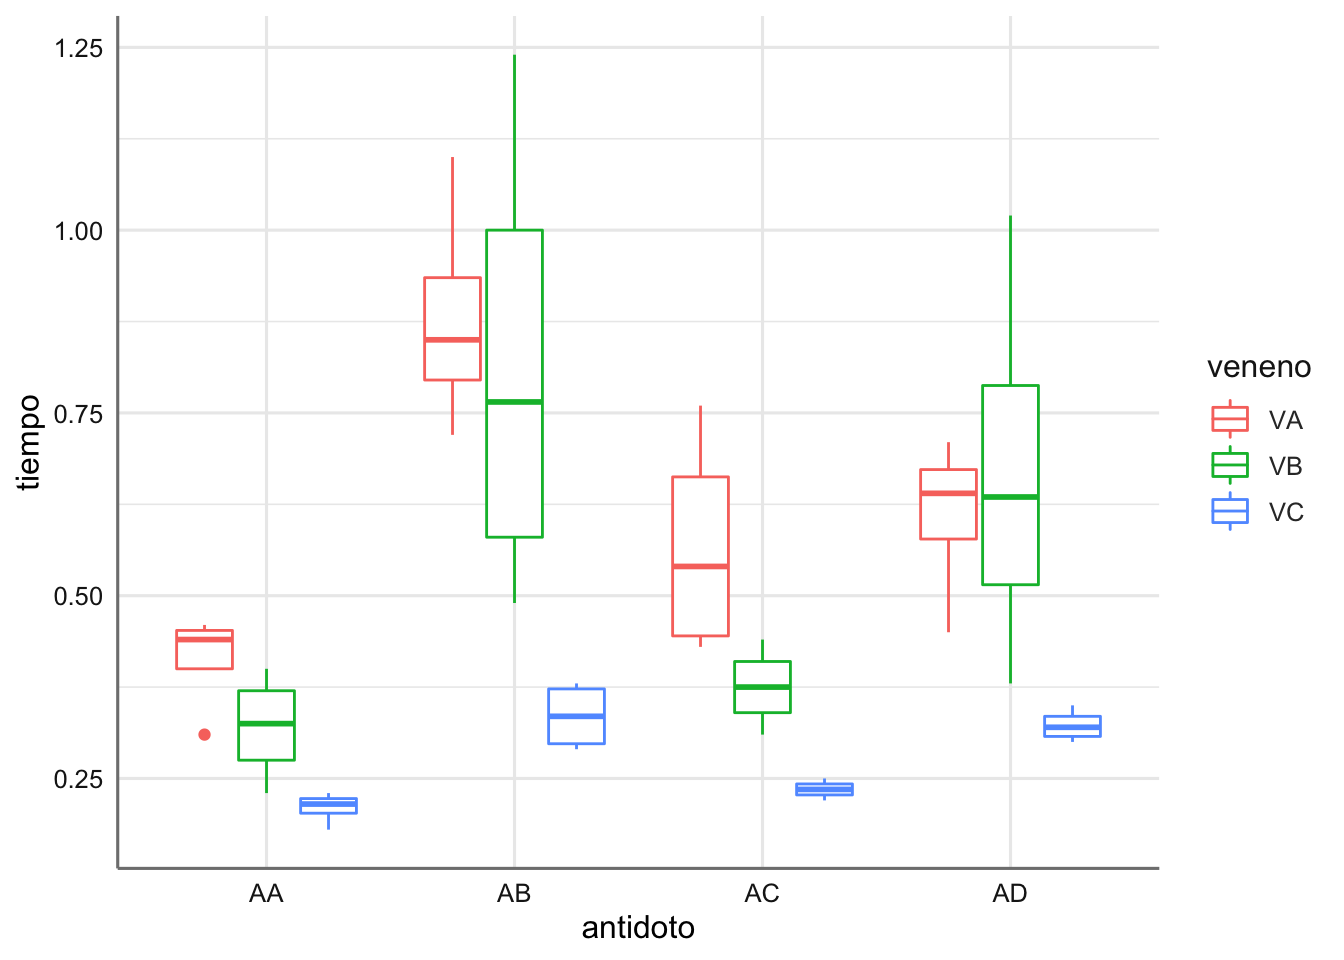
\includegraphics{libroSTAT_files/figure-latex/unnamed-chunk-3-1.pdf}

A la vista de la Figura anterior se puede apreciar que el comportamiento del tiempo de vida con repecto a la velocidad disminuye al aumentar esta última, y además ese decenso es distinto en función de la herramienta utilizada. A la misma velocidad la herramienta A proporciona un tiempo de vida inferior que la herramienta B. Para ambas máquinas se aprecía una tendencia lineal bastante clara que deberá ser objeto de estudio. Esto implicaría que nuestro modelo se desdoblaría en dos rectas de regresión lineal simple en función de la herramienta utilizada.

\BeginKnitrBlock{example}[Longevidad]
\protect\hypertarget{exm:acov02}{}{\label{exm:acov02} \iffalse (Longevidad) \fi{} }Partridge y Farquhar realizan un experimento para relacionar la vida útil (\texttt{longevidad}) de las moscas de la fruta con su actividad sexual (\texttt{actividad}). La información recogida es la longevidad en días de 125 moscas macho, divididas en cinco grupos bajo diferentes condiciones ambientales para medir su actividad sexual. Asimismo, se recoge la longitud del tórax (\texttt{thorax}) ya que se sospecha que afecta directamente a la longevidad de las moscas.
\EndKnitrBlock{example}

Cargamos los datos y realizamos el gráfico descriptivo:

\begin{Shaded}
\begin{Highlighting}[]
\CommentTok{# Carga de datos}
\NormalTok{thorax <-}\StringTok{ }\KeywordTok{c}\NormalTok{(}\FloatTok{0.68}\NormalTok{, }\FloatTok{0.68}\NormalTok{, }\FloatTok{0.72}\NormalTok{, }\FloatTok{0.72}\NormalTok{, }\FloatTok{0.76}\NormalTok{, }\FloatTok{0.76}\NormalTok{, }
            \FloatTok{0.76}\NormalTok{, }\FloatTok{0.76}\NormalTok{, }\FloatTok{0.76}\NormalTok{, }\FloatTok{0.8}\NormalTok{, }\FloatTok{0.8}\NormalTok{, }\FloatTok{0.8}\NormalTok{, }\FloatTok{0.84}\NormalTok{, }\FloatTok{0.84}\NormalTok{, }\FloatTok{0.84}\NormalTok{, }\FloatTok{0.84}\NormalTok{, }\FloatTok{0.84}\NormalTok{, }\FloatTok{0.84}\NormalTok{, }\FloatTok{0.88}\NormalTok{, }\FloatTok{0.88}\NormalTok{, }\FloatTok{0.92}\NormalTok{, }\FloatTok{0.92}\NormalTok{, }\FloatTok{0.92}\NormalTok{, }\FloatTok{0.94}\NormalTok{, }\FloatTok{0.64}\NormalTok{, }\FloatTok{0.7}\NormalTok{, }\FloatTok{0.72}\NormalTok{, }\FloatTok{0.72}\NormalTok{, }\FloatTok{0.72}\NormalTok{, }\FloatTok{0.76}\NormalTok{, }\FloatTok{0.78}\NormalTok{, }\FloatTok{0.8}\NormalTok{, }\FloatTok{0.84}\NormalTok{, }\FloatTok{0.84}\NormalTok{, }\FloatTok{0.84}\NormalTok{, }\FloatTok{0.84}\NormalTok{, }\FloatTok{0.84}\NormalTok{, }\FloatTok{0.88}\NormalTok{, }\FloatTok{0.88}\NormalTok{, }\FloatTok{0.88}\NormalTok{, }\FloatTok{0.88}\NormalTok{, }\FloatTok{0.88}\NormalTok{, }\FloatTok{0.92}\NormalTok{, }\FloatTok{0.92}\NormalTok{, }\FloatTok{0.92}\NormalTok{, }\FloatTok{0.92}\NormalTok{, }\FloatTok{0.92}\NormalTok{, }\FloatTok{0.92}\NormalTok{, }\FloatTok{0.94}\NormalTok{, }\FloatTok{0.64}\NormalTok{, }\FloatTok{0.68}\NormalTok{, }\FloatTok{0.72}\NormalTok{, }\FloatTok{0.76}\NormalTok{, }\FloatTok{0.76}\NormalTok{, }\FloatTok{0.8}\NormalTok{, }\FloatTok{0.8}\NormalTok{, }\FloatTok{0.8}\NormalTok{, }\FloatTok{0.82}\NormalTok{, }\FloatTok{0.82}\NormalTok{, }\FloatTok{0.84}\NormalTok{, }\FloatTok{0.84}\NormalTok{, }\FloatTok{0.84}\NormalTok{, }\FloatTok{0.84}\NormalTok{, }\FloatTok{0.84}\NormalTok{, }\FloatTok{0.84}\NormalTok{, }\FloatTok{0.88}\NormalTok{, }\FloatTok{0.88}\NormalTok{, }\FloatTok{0.88}\NormalTok{, }\FloatTok{0.88}\NormalTok{, }\FloatTok{0.88}\NormalTok{, }\FloatTok{0.88}\NormalTok{, }\FloatTok{0.88}\NormalTok{, }\FloatTok{0.92}\NormalTok{, }\FloatTok{0.92}\NormalTok{, }\FloatTok{0.68}\NormalTok{, }\FloatTok{0.68}\NormalTok{, }\FloatTok{0.72}\NormalTok{, }\FloatTok{0.76}\NormalTok{, }\FloatTok{0.78}\NormalTok{, }\FloatTok{0.8}\NormalTok{, }\FloatTok{0.8}\NormalTok{, }\FloatTok{0.8}\NormalTok{, }\FloatTok{0.84}\NormalTok{,  }\FloatTok{0.84}\NormalTok{, }\FloatTok{0.84}\NormalTok{, }\FloatTok{0.84}\NormalTok{, }\FloatTok{0.84}\NormalTok{, }\FloatTok{0.84}\NormalTok{, }\FloatTok{0.88}\NormalTok{, }\FloatTok{0.88}\NormalTok{, }\FloatTok{0.88}\NormalTok{, }\FloatTok{0.9}\NormalTok{, }\FloatTok{0.9}\NormalTok{, }\FloatTok{0.9}\NormalTok{, }\FloatTok{0.9}\NormalTok{, }\FloatTok{0.9}\NormalTok{, }\FloatTok{0.9}\NormalTok{, }\FloatTok{0.92}\NormalTok{, }\FloatTok{0.92}\NormalTok{, }\FloatTok{0.64}\NormalTok{, }\FloatTok{0.64}\NormalTok{, }\FloatTok{0.68}\NormalTok{, }\FloatTok{0.72}\NormalTok{, }\FloatTok{0.72}\NormalTok{, }\FloatTok{0.74}\NormalTok{, }\FloatTok{0.76}\NormalTok{, }\FloatTok{0.76}\NormalTok{, }\FloatTok{0.76}\NormalTok{, }\FloatTok{0.78}\NormalTok{, }\FloatTok{0.8}\NormalTok{, }\FloatTok{0.8}\NormalTok{, }\FloatTok{0.82}\NormalTok{, }\FloatTok{0.82}\NormalTok{, }\FloatTok{0.84}\NormalTok{, }\FloatTok{0.84}\NormalTok{, }\FloatTok{0.84}\NormalTok{, }\FloatTok{0.84}\NormalTok{, }\FloatTok{0.88}\NormalTok{, }\FloatTok{0.88}\NormalTok{, }\FloatTok{0.88}\NormalTok{, }\FloatTok{0.88}\NormalTok{, }\FloatTok{0.88}\NormalTok{, }\FloatTok{0.88}\NormalTok{, }\FloatTok{0.92}\NormalTok{)}
\NormalTok{longevidad <-}\StringTok{ }\KeywordTok{c}\NormalTok{(}\DecValTok{37}\NormalTok{, }\DecValTok{49}\NormalTok{,  }\DecValTok{46}\NormalTok{,  }\DecValTok{63}\NormalTok{,  }\DecValTok{39}\NormalTok{,  }\DecValTok{46}\NormalTok{,  }\DecValTok{56}\NormalTok{,  }\DecValTok{63}\NormalTok{,  }\DecValTok{65}\NormalTok{,  }\DecValTok{56}\NormalTok{,  }\DecValTok{65}\NormalTok{,  }\DecValTok{70}\NormalTok{,  }\DecValTok{63}\NormalTok{,  }\DecValTok{65}\NormalTok{, }\DecValTok{70}\NormalTok{,  }\DecValTok{77}\NormalTok{,  }\DecValTok{81}\NormalTok{,  }\DecValTok{86}\NormalTok{,  }\DecValTok{70}\NormalTok{,  }\DecValTok{70}\NormalTok{,  }\DecValTok{77}\NormalTok{,  }\DecValTok{77}\NormalTok{,  }\DecValTok{81}\NormalTok{,  }\DecValTok{77}\NormalTok{,  }\DecValTok{40}\NormalTok{,  }\DecValTok{37}\NormalTok{,  }\DecValTok{44}\NormalTok{, }\DecValTok{47}\NormalTok{,  }\DecValTok{47}\NormalTok{,  }\DecValTok{47}\NormalTok{,  }\DecValTok{68}\NormalTok{,  }\DecValTok{47}\NormalTok{,  }\DecValTok{54}\NormalTok{,  }\DecValTok{61}\NormalTok{,  }\DecValTok{71}\NormalTok{,  }\DecValTok{75}\NormalTok{,  }\DecValTok{89}\NormalTok{,  }\DecValTok{58}\NormalTok{,  }\DecValTok{59}\NormalTok{,  }\DecValTok{62}\NormalTok{, }\DecValTok{79}\NormalTok{,  }\DecValTok{96}\NormalTok{,  }\DecValTok{58}\NormalTok{,  }\DecValTok{62}\NormalTok{,  }\DecValTok{70}\NormalTok{,  }\DecValTok{72}\NormalTok{,  }\DecValTok{75}\NormalTok{,  }\DecValTok{96}\NormalTok{,  }\DecValTok{75}\NormalTok{,  }\DecValTok{46}\NormalTok{,  }\DecValTok{42}\NormalTok{,  }\DecValTok{65}\NormalTok{,  }\DecValTok{46}\NormalTok{, }\DecValTok{58}\NormalTok{,  }\DecValTok{42}\NormalTok{,  }\DecValTok{48}\NormalTok{,  }\DecValTok{58}\NormalTok{,  }\DecValTok{50}\NormalTok{,  }\DecValTok{80}\NormalTok{,  }\DecValTok{63}\NormalTok{,  }\DecValTok{65}\NormalTok{,  }\DecValTok{70}\NormalTok{,  }\DecValTok{70}\NormalTok{,  }\DecValTok{72}\NormalTok{,  }\DecValTok{97}\NormalTok{,  }\DecValTok{46}\NormalTok{, }\DecValTok{56}\NormalTok{,  }\DecValTok{70}\NormalTok{,  }\DecValTok{70}\NormalTok{,  }\DecValTok{72}\NormalTok{,  }\DecValTok{76}\NormalTok{,  }\DecValTok{90}\NormalTok{,  }\DecValTok{76}\NormalTok{,  }\DecValTok{92}\NormalTok{,  }\DecValTok{21}\NormalTok{,  }\DecValTok{40}\NormalTok{,  }\DecValTok{44}\NormalTok{,  }\DecValTok{54}\NormalTok{,  }\DecValTok{36}\NormalTok{, }\DecValTok{40}\NormalTok{,  }\DecValTok{56}\NormalTok{,  }\DecValTok{60}\NormalTok{,  }\DecValTok{48}\NormalTok{,  }\DecValTok{53}\NormalTok{,  }\DecValTok{60}\NormalTok{,  }\DecValTok{60}\NormalTok{,  }\DecValTok{65}\NormalTok{,  }\DecValTok{68}\NormalTok{,  }\DecValTok{60}\NormalTok{,  }\DecValTok{81}\NormalTok{,  }\DecValTok{81}\NormalTok{,  }\DecValTok{48}\NormalTok{, }\DecValTok{48}\NormalTok{,  }\DecValTok{56}\NormalTok{,  }\DecValTok{68}\NormalTok{,  }\DecValTok{75}\NormalTok{,  }\DecValTok{81}\NormalTok{,  }\DecValTok{48}\NormalTok{,  }\DecValTok{68}\NormalTok{,  }\DecValTok{16}\NormalTok{,  }\DecValTok{19}\NormalTok{,  }\DecValTok{19}\NormalTok{,  }\DecValTok{32}\NormalTok{,  }\DecValTok{33}\NormalTok{,  }\DecValTok{33}\NormalTok{, }\DecValTok{30}\NormalTok{,  }\DecValTok{42}\NormalTok{,  }\DecValTok{42}\NormalTok{,  }\DecValTok{33}\NormalTok{,  }\DecValTok{26}\NormalTok{,  }\DecValTok{30}\NormalTok{,  }\DecValTok{40}\NormalTok{,  }\DecValTok{54}\NormalTok{,  }\DecValTok{34}\NormalTok{,  }\DecValTok{34}\NormalTok{,  }\DecValTok{47}\NormalTok{,  }\DecValTok{47}\NormalTok{,  }\DecValTok{42}\NormalTok{, }\DecValTok{47}\NormalTok{,  }\DecValTok{54}\NormalTok{,  }\DecValTok{54}\NormalTok{,  }\DecValTok{56}\NormalTok{,  }\DecValTok{60}\NormalTok{,  44L)}
\NormalTok{actividad <-}\StringTok{ }\KeywordTok{c}\NormalTok{(}\KeywordTok{rep}\NormalTok{(}\StringTok{"G1"}\NormalTok{,}\DecValTok{24}\NormalTok{),}\KeywordTok{rep}\NormalTok{(}\StringTok{"G2"}\NormalTok{,}\DecValTok{25}\NormalTok{),}\KeywordTok{rep}\NormalTok{(}\StringTok{"G3"}\NormalTok{,}\DecValTok{25}\NormalTok{),}\KeywordTok{rep}\NormalTok{(}\StringTok{"G4"}\NormalTok{,}\DecValTok{25}\NormalTok{),}\KeywordTok{rep}\NormalTok{(}\StringTok{"G5"}\NormalTok{,}\DecValTok{25}\NormalTok{))}
\NormalTok{longevidad <-}\StringTok{ }\KeywordTok{data.frame}\NormalTok{(thorax,longevidad,actividad)}
\CommentTok{# Gráfico}
\KeywordTok{ggplot}\NormalTok{(longevidad, }\KeywordTok{aes}\NormalTok{(}\DataTypeTok{x =}\NormalTok{ thorax, }\DataTypeTok{y =}\NormalTok{ longevidad, }\DataTypeTok{color =}\NormalTok{ actividad)) }\OperatorTok{+}\StringTok{ }
\StringTok{  }\KeywordTok{geom_point}\NormalTok{() }
\end{Highlighting}
\end{Shaded}

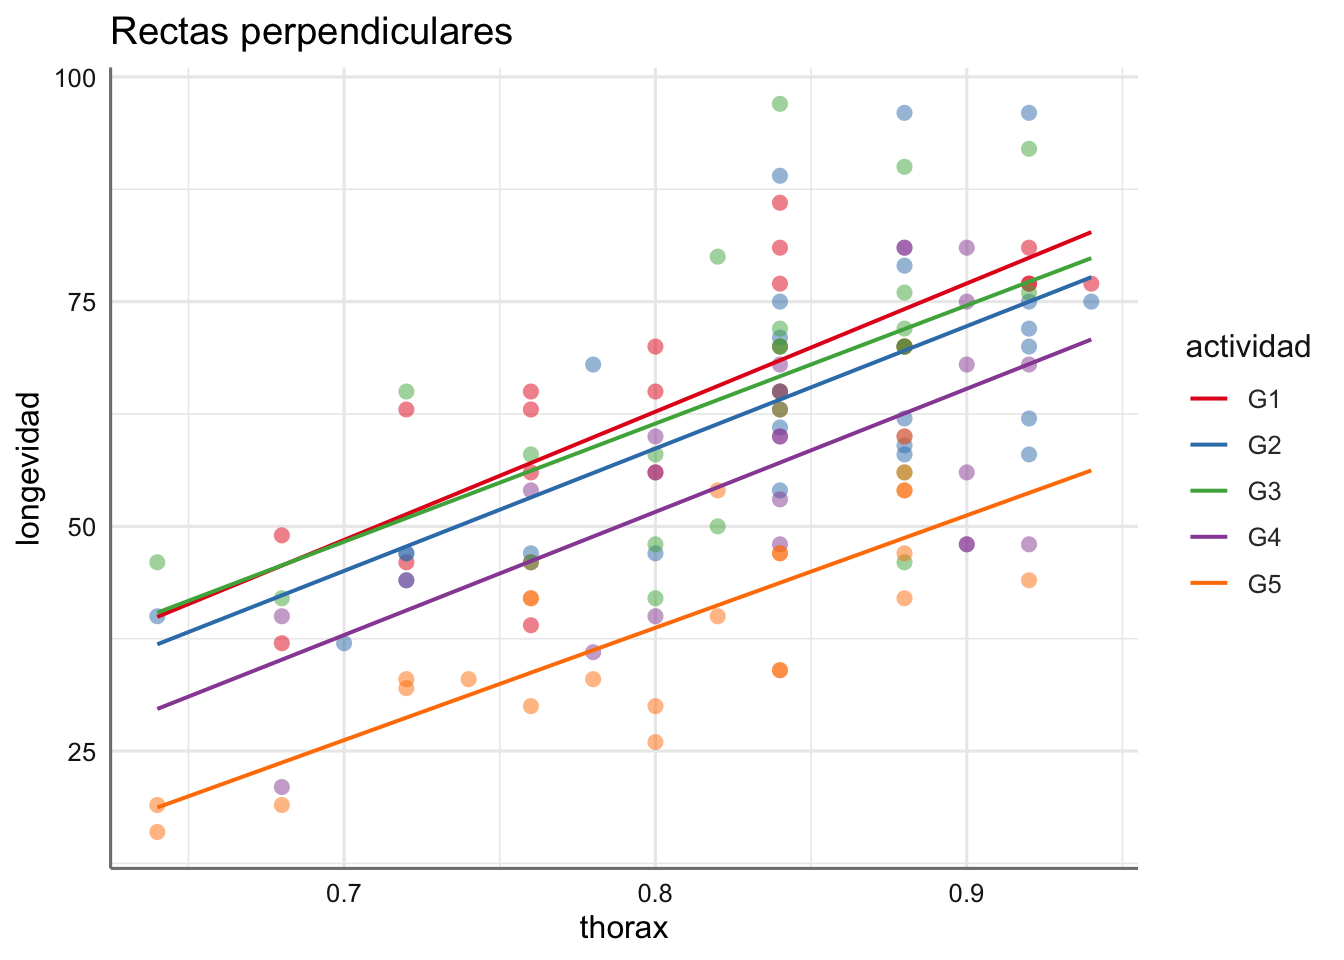
\includegraphics{libroSTAT_files/figure-latex/unnamed-chunk-4-1.pdf}

Se puede ver como la longevidad aumenta caundo aumenta la longitud del thorax pero ese crecimiento no parece distinto según actividad, dado que las nuebes de puntos están bastante mezcladas. En este caso no prece adecuado un modelo lineal para cada grupo de actividad.

\hypertarget{modelo-ancova}{%
\section{Modelo ANCOVA}\label{modelo-ancova}}

Consideramos el modelo ANCOVA más sencillo donde consideramos dos variables predictoras: una numérica y otra un factor. Consideramos una muestra de tamaño \(n\) donde tenemos:

\begin{itemize}
\tightlist
\item
  Una variable respuesta, \(Y\), de tipo numérico con observaciones \(y_1,...,y_n\).
\item
  Una variable predictora, \(X\), de tipo numérico con observaciones \(x_1,...,x_n\).
\item
  Una variable predictora, \(F\), de tipo categórico con \(I\) grupos o niveles distintos de tamaños muestrales \(n_1,n_2,...,n_I\), de forma que \(n = n_1 + n_2 + ... + n_I\), de forma que el vector de observaciones de la respuesta y de la predictora numérica se pueden escribir como:
  \[
  (Y_1, Y_2,...,Y_I) = y_{11},\ldots,y_{1n_1},y_{21},\ldots,y_{2n_2},\ldots,y_{I1},\ldots,y_{In_I}
  \]
  \[
  (X_1, X_2,...,X_I) = x_{11},\ldots,x_{1n_1},x_{21},\ldots,x_{2n_2},\ldots,x_{I1},\ldots,x_{In_I}
  \]
  donde el primer subíndice indica el nivel del factor y el segundo la posición dentro del conjunto de datos de dicho nivel del factor.
\item
  Conjunto \(\mu_i\) de medias de todas las observaciones de la respuesta asociadas con el nivel \(i\) del factor, es decir:
\end{itemize}

\[
\mu_i = \frac{\sum_{j = 1}^{n_j} y_{ij}}{n_i}; \text{ i = 1, 2,..., I}
\]

\begin{itemize}
\tightlist
\item
  Media global de la respuesta, \(\mu\), que se puede obtener como:
\end{itemize}

\[
\mu = \frac{\sum_{j = 1}^{I} \mu_{j}}{I}
\]

\begin{itemize}
\tightlist
\item
  Incrementos, \(\alpha_i\), de cada una de las medias de cada grupo con respecto a la media global, es decir:
\end{itemize}

\[
\alpha_i= \mu - \mu_i; \text{ i = 1, 2,..., I}
\]

\begin{itemize}
\item
  Pendiente común, \(\beta\), que representa la posible relación entre las variables de tipo numérico.
\item
  Pendientes diferentes entre las predictoras numéricas asociadas a cada nivel del factor, \(\gamma_i\) con \(i = 1,...,I\).
\end{itemize}

En esta situación el modelo que describe la posible relación entre respuesta y predictoras se puede escribir como:
\begin{equation}
y_{ij} = \alpha_0 + \alpha_i + \beta x_{ij} + \gamma_i x_{ij} + \epsilon_{ij};\quad  i=1,...,I \quad \text{con} \quad \alpha_I = 0
\label{eq:ancova}
\end{equation}

Que en forma matricial se puede escribir fácilmente (de forma análoga al ANOVA de un vía) sin más que considerar \(1_(n_i )={1,...,1}\) un vector de \(n_i\) unos, \(0_(n_i )={0,...,0}\) un vector de \(n_i\) ceros, para cada uno de los niveles i del factor la matriz de diseño viene dada por:
\[
Y = \left( 
\begin{array}{c}
   Y_1 \\
   Y_2 \\
   \ldots \\
   Y_I \\
\end{array}
\right)
=
\left( 
\begin{array}{ccccccccc}
   1_{n_1} & 1_{n_1} & 0_{n_1} & \ldots & 0_{n_1} & X_1 & X_1 & \ldots & 0_{n_1}\\
   1_{n_2} & 0_{n_2} & 1_{n_2} & \ldots & 0_{n_2} & X_2 & 0_{n_2} & \ldots & 0_{n_2}\\
   \ldots & \ldots & \ldots & \ldots & \ldots & \ldots & \ldots & \ldots & 0_{n_3}\\
   1_{n_I} & 0_{n_I} & 0_{n_I} &\ldots & 1_{n_I} & X_I & 0_{n_I} & \ldots & X_I\\
\end{array}
\right)
\left( 
\begin{array}{c}
   \alpha_0 \\
   \alpha_1 \\
  \alpha_2 \\
 \ldots \\
   \alpha_{I_1} \\
   \beta \\
   \gamma_1\\
   \ldots\\
   \gamma_I\\
\end{array}
\right)
+
\left( 
\begin{array}{c}
   e_1 \\
   e_2 \\
   \ldots \\
   e_n \\
\end{array}
\right) = X\beta + \epsilon
\]

donde las primeras \(I\) columnas representan el efecto del factor (ANOVA de una vía), la siguiente columna representa el efecto común entre predictoras numéricas (Regresión lineal simple), y las últimas \(I\) columnas representan el efecto distinto de la predictora numérica para cada nivel del factor. Estas columnas se obtienen fácilmente multiplicando la columna de \(X\) por cada de las columnas desde la \(2\) a la \(I\).

Las posibles modelos anidados que se pueden obtener a partir de la ecuación \eqref{eq:ancova}, así como sus interpretaciones se presentan a continuación. Además se ofrece la interpretación de dichos modelos en términos de los coeficientes que resulten significativos. La estructura secuencial de contrastes pasa por estudiar si debemos considerar una pendiente distinta para la predictora numérica en función de los niveles del factor, que es equivalente a plantear el contraste:

\begin{equation}
\left\{ 
\begin{array}{ll}
H_0: & \gamma_1 = \gamma_2 = \ldots = \gamma_I = 0\\
H_a: & \mbox{Al menos hay una pendiente distinto de cero}\\
\end{array}
\right.
\label{eq:contraste1}
\end{equation}

\begin{itemize}
\tightlist
\item
  Si rechazamos el contraste \eqref{eq:contraste1} tendremos un modelo de regresión entre la respuesta y la predictora numérica para cada nivel del factor, es decir, I rectas de regresión distintas con ecuaciones:
\end{itemize}

\begin{equation}
\begin{array}{ll}
y_{1j} &= (\alpha_0 + \alpha_1) + (\beta + \gamma_1) x_{1j} + \epsilon_{1j}\\
y_{2j} &= (\alpha_0 + \alpha_2) + (\beta + \gamma_2) x_{2j} + \epsilon_{2j}\\
\ldots &= \ldots \\
y_{Ij} &= (\alpha_0 + \alpha_I) + (\beta + \gamma_I) x_{Ij} + \epsilon_{Ij}\\
\end{array}
\label{eq:modeloancovaconinteraccion}
\end{equation}

con interceptaciones \(\alpha_0 + \alpha_i\) y pendientes \(\beta + \gamma_i\) para cada uno de los \(I\) niveles del factor. Tenemos I modelos de regresión distintos (uno por cada nivel del factor), es decir, tenemos I rectas perpendiculares o que se cortan.

\begin{itemize}
\tightlist
\item
  Si no rechazamos el contraste \eqref{eq:contraste1} tendremos un único modelo de regresión entre la respuesta y la predictora pero con diferentes interceptaciones (la pendiente es la misma), es decir, I rectas paralelas cuyas ecuaciones vienen dadas por:
\end{itemize}

\begin{equation}
\begin{array}{ll}
y_{1j} &= (\alpha_0 + \alpha_1) + \beta  x_{1j} + \epsilon_{1j}\\
y_{2j} &= (\alpha_0 + \alpha_2) + \beta  x_{2j} + \epsilon_{2j}\\
\ldots &= \ldots \\
y_{Ij} &= (\alpha_0 + \alpha_I) + \beta  x_{Ij} + \epsilon_{Ij}\\
\end{array}
\label{eq:modeloancovasininteraccion}
\end{equation}

En la situación donde el contraste \eqref{eq:contraste1} es no significativo podemos definir diferentes modelos anidados en función de los incrementos del factor (\alpha`s) y la pendiente \(\beta\). Los contrates son:

\begin{equation}
\left\{ 
\begin{array}{ll}
H_0: & \alpha_1 = \alpha_2 = \ldots = \alpha_I = 0\\
H_a: & \mbox{Al menos hay un incremento distinto de cero}\\
\end{array}
\right.
\label{eq:contraste2}
\end{equation}
y
\begin{equation}
\left\{ 
\begin{array}{ll}
H_0: & \beta = 0\\
H_a: & \beta \neq 0
\end{array}
\right.
\label{eq:contraste3}
\end{equation}

\begin{itemize}
\tightlist
\item
  Si rechazamos la hipótesis nula de \eqref{eq:contraste2} pero no rechazamos la hipótesis nula de \eqref{eq:contraste3} diríamos que no hay efecto de la predictora numérica pero que si podemos establecer diferencias entre las medias de la respuesta dadas por los diferentes niveles del factor (Modelo ANOVA con ecuaciones \eqref{eq:modelomedias}.
\item
  Si no rechazamos la hipótesis nula de \eqref{eq:contraste2} pero si rechazamos la hipótesis nula de \eqref{eq:contraste3} diríamos que no hay efecto del factor pero si que podemos establecer un modelo de regresión entre la respuesta y la predictora numérica (Modelo de Regresión Lineal Simple con ecuación \eqref{eq:modeloregresion}).
\item
  Si no rechazamos la hipótesis nula de \eqref{eq:contraste2} y no rechazamos la hipótesis nula de \eqref{eq:contraste3} estaríamos ante un modelo nulo donde el comportamiento de la respuesta no viene explicado por las predictoras consideradas.
\end{itemize}

Las ecuaciones de los modelos resultantes son:

\begin{itemize}
\tightlist
\item
  Modelo ANOVA:
\end{itemize}

\begin{equation}
\begin{array}{ll}
y_{1j} &= (\alpha_0 + \alpha_1) + \epsilon_{1j}\\
y_{2j} &= (\alpha_0 + \alpha_2) + \epsilon_{2j}\\
\ldots &= \ldots \\
y_{Ij} &= (\alpha_0 + \alpha_I) + \epsilon_{Ij}\\
\end{array}
\label{eq:modelomedias}
\end{equation}

\begin{itemize}
\tightlist
\item
  Modelo de Regresión Lineal Simple:
\end{itemize}

\begin{equation}
\begin{array}{ll}
y_{ij} &= \alpha_0 + \beta  x_{ij} + \epsilon_{ij}\\
\end{array}
\label{eq:modeloregresion}
\end{equation}

Atendiendo a las ecuaciones obtenidas las posible modelizaciones resultantes del modelo saturado son:

\begin{itemize}
\tightlist
\item
  I rectas que se cortan (modelo con interacción factor - numérica \eqref{eq:modeloancovaconinteraccion}).
\item
  I rectas paralelas (modelo sin interacción pero con factor y numérica \eqref{eq:modeloancovasininteraccion}).
\item
  Una recta de regresión (modelo con la predictora numérica únicamente \eqref{eq:modeloregresion}).
\item
  Diferencias entre las medias (modelo con el factor únicamente \eqref{eq:modelomedias})
\end{itemize}

Vemos gráficamente los posibles modelos que podemos construir sobre los dos ejemplos presentados anteriormente:

\begin{itemize}
\tightlist
\item
  Datos de tiempo de vida: ¿Cómo interpretamos los gráficos obtenidos?
\end{itemize}

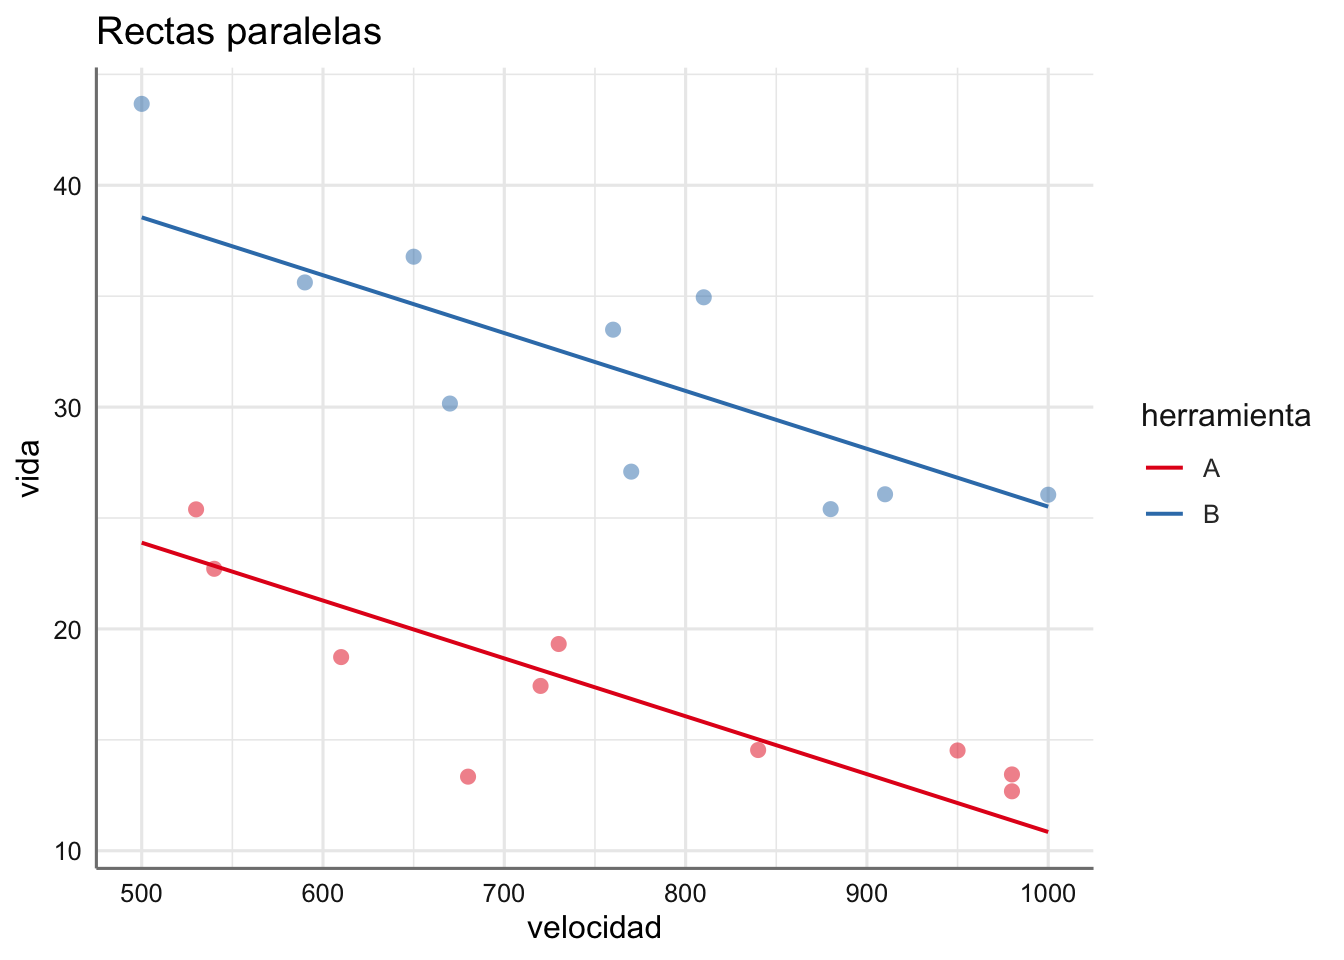
\includegraphics{libroSTAT_files/figure-latex/unnamed-chunk-5-1.pdf} \includegraphics{libroSTAT_files/figure-latex/unnamed-chunk-5-2.pdf} \includegraphics{libroSTAT_files/figure-latex/unnamed-chunk-5-3.pdf} \includegraphics{libroSTAT_files/figure-latex/unnamed-chunk-5-4.pdf}

\begin{itemize}
\tightlist
\item
  Datos de longevidad: ¿Cómo interpretamos los gráficos obtenidos?
\end{itemize}

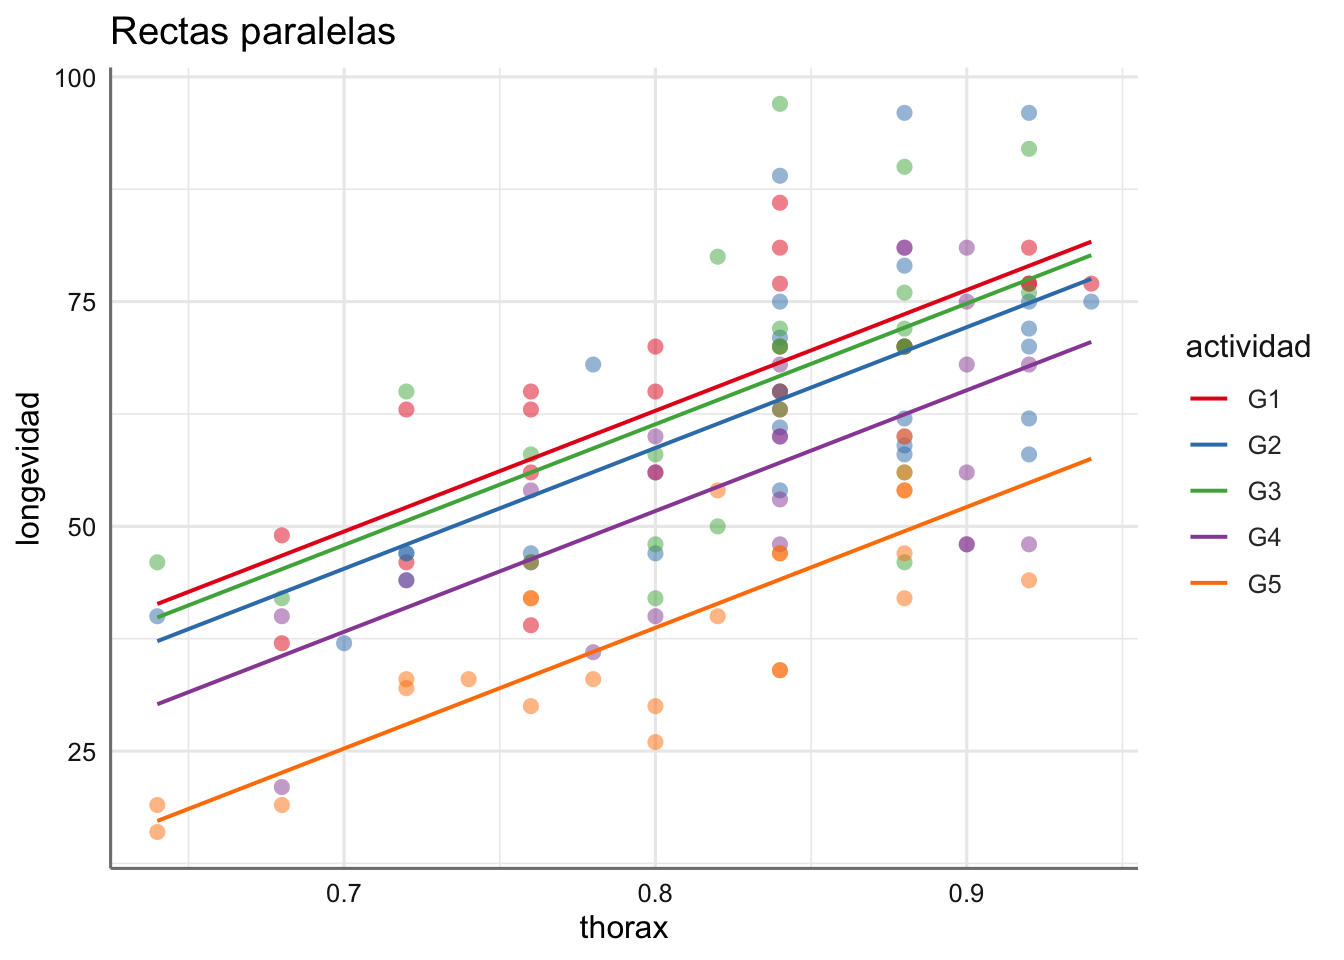
\includegraphics{libroSTAT_files/figure-latex/unnamed-chunk-6-1.pdf} \includegraphics{libroSTAT_files/figure-latex/unnamed-chunk-6-2.pdf} \includegraphics{libroSTAT_files/figure-latex/unnamed-chunk-6-3.pdf} \includegraphics{libroSTAT_files/figure-latex/unnamed-chunk-6-4.pdf}

Las hipótesis de este modelo es que los errores se distribuyen de forma independiente mediante una distribución Normal de media cero y varianza constante \(\sigma^2\) para cada uno de los grupos que determina la variable predictora. Estas hipótesis se adaptarán en función del tipo de modelo que finalmente alcanzemos en el proceso de contraste. Todos ellos se pueden resolver mediante un test \(F\), y más adelante veremos como construir la secuencia de modelos para decidir sobre el modelo final.

\hypertarget{especificaciuxf3n-del-modelo-en-r}{%
\section{\texorpdfstring{Especificación del modelo en \texttt{R}}{Especificación del modelo en R}}\label{especificaciuxf3n-del-modelo-en-r}}

El modelo ANCOVA planteado en el punto anterior para un factor F y una variable predictora numérica X, se puede escribir en R en su formato reducido como:

\[Y \sim F + X + F:X\]

donde:

\begin{itemize}
\tightlist
\item
  \(F\) representa el efecto del factor, es decir, comparamos si las medias de la respuesta para cada grupo pueden considerarse iguales.
\item
  \(X\) representa el efecto de regresión asociado con la variable numérica, es decir, la respuesta y X están relacionadas mediante una única pendiente que deberemos estimar.
\item
  \(F:X\) representa el efecto de interacción entre predictoras, es decir, que la respuesta se relaciona con la predictora numérica mediante tantas curvas (generalmente líneas) como niveles tenga el factor \(F\).
\end{itemize}

A continuación se presentan los modelos reducidos para diferentes situaciones experimentales en el número y tipo de varaibles predictoras:

\begin{itemize}
\tightlist
\item
  Modelo para dos factores (\(F_1\) y \(F_2\)) y una numérica (\(X\))
\end{itemize}

\[Y \sim F_1 + F_2 + F_1:F_2 + X + F_1:X + F_2:X + F_1:F_2:X\]
o en forma más simplificada \(Y \sim F_1*F_2*X\)

\begin{itemize}
\tightlist
\item
  Modelo para un factor (\(F\)) y dos numéricas (\(X_1\) y \(X_2\))
\end{itemize}

\[Y \sim F + X_1 + X_2 + F:X_1 + F:X_2\]
o en forma más simplificada \(Y \sim F*(X_1 + X_2)\)

\begin{itemize}
\tightlist
\item
  Modelo para dos factores (\(F_1\) y \(F_2\)) y dos numéricas (\(X_1\) y \(X_2\))
\end{itemize}

\[Y \sim F_1*F_2*(X_1 + X_2)\]

Como se puede ver la complejidad del modelo aumenta sustancialmente con la consideración de más variables predictoras. La forma de expresar el modleo saturado debe contemplar tanto os efectos principales asociados a cada predictora, como los efectos de interacción entre factores y entre factores y numéricas.

\hypertarget{estimaciuxf3n-y-selecciuxf3n-del-modelo}{%
\section{Estimación y Selección del modelo}\label{estimaciuxf3n-y-selecciuxf3n-del-modelo}}

Dado que hemos expresado el modelo ANCOVA como un modelo de tipo lineal con una ecuación similar a los modelos de regresión múltiple, la estimación de los parámetros del modelo se puede realizar utilizando las ecuaciones normales. En el proceso de selección del mejor modelo actuaremos como en los modelos ANOVA, es decir partiremos del modelo saturado y veremos que efectos puede ser considerados como irrelevantes, y por tanto deben desaparecer del modelo. Esta selección nos permitirá elegir el modelo final resultante. En este caso más sencillo podemos escribir todos los modelos posibles y elegir el mejor de ellos, bien mediante la comparación con el test F o con el AIC, pero veremos como utilizar los procedimientos secuenciales automáticos para problemas más complejos.

\hypertarget{ejemplos}{%
\subsection{Ejemplos}\label{ejemplos}}

Realizamos la selección y estimación del mejor modelo para cada uno de los conjuntos de datos considerados.

\hypertarget{datos-de-tiempo-de-vida}{%
\subsubsection{Datos de tiempo de vida}\label{datos-de-tiempo-de-vida}}

Construímos el modelo saturado y seleccionamos mediante el test \(F\).

\begin{verbatim}
## 
## 
##                                  Elimination Summary                                  
## -------------------------------------------------------------------------------------
##         Variable                               Adj.                                      
## Step           Removed           R-Square    R-Square     C(p)       AIC        RMSE     
## -------------------------------------------------------------------------------------
##    1    velocidad:herramienta      0.8969      0.8847    3.9652    106.6591    3.0919    
## -------------------------------------------------------------------------------------
\end{verbatim}

El proceso de selección identifica el efecto de interacción entre \texttt{velocidad} y \texttt{herramienta} como no significativo, de forma que el modelo final viene dado por:
\[vida \sim velocidad + herramienta\]
Ajustamos el modelo y estudiamos los parámetros obtenidos:

~

vida

Predictors

Estimates

CI

(Intercept)

36.93

29.56~--~44.30

velocidad

-0.03

-0.04~--~-0.02

herramienta {[}B{]}

14.67

11.75~--~17.58

Observations

20

En este caso tenemos un modelo con dos rectas paralelas (una por cada tipo de herramienta) cuyas ecuaciones de estimación vienen dadas por:

\[
\left\{ 
\begin{array}{lll}
\mbox{Herramienta A}:& \widehat{Vida_{A}} = 36.93 + 0  + 14.67*velocidad &= 36.93 + 14.67*velocidad\\
\mbox{Herramienta B}:& \widehat{Vida_{B}} = 36.93 - 0.03 + 14.67*velocidad &= 36.90 + 14.67*velocidad \\
\end{array}
\right.
\]

Tenemos una interceptación mayor para la herramienta A indicando que la recta asociada con dicha herramienta está por encima de la de la herramienta B. Además, la pendiente negativa asociada con la velocidad indica que conforme aumenta esta disminuye el tiempo de vida. Ese efecto es mayor si usamos la herramienta de tipo B dado que la recta ajustada está por debajo de la de la herramienta A.

\hypertarget{datos-de-longevidad}{%
\subsubsection{Datos de longevidad}\label{datos-de-longevidad}}

Construímos el modelo saturado y seleccionamos mediante el test \(F\).

\begin{verbatim}
## 
## 
##                                Elimination Summary                                 
## ----------------------------------------------------------------------------------
##         Variable                          Adj.                                        
## Step        Removed         R-Square    R-Square     C(p)        AIC        RMSE      
## ----------------------------------------------------------------------------------
##    1    thorax:actividad      0.6527       0.638    -3.7881    943.8165    10.5394    
## ----------------------------------------------------------------------------------
\end{verbatim}

El proceso de selección identifica el efecto de interacción entre \texttt{thorax} y \texttt{actividad} como no significativo, de forma que el modelo final viene dado por:
\[longevidad \sim thorax + actividad\]
Ajustamos el modelo y estudiamos los parámetros obtenidos:

~

longevidad

Predictors

Estimates

CI

(Intercept)

-44.61

-65.53~--~-23.69

thorax

134.34

109.13~--~159.55

actividad {[}G2{]}

-4.14

-10.13~--~1.86

actividad {[}G3{]}

-1.50

-7.48~--~4.47

actividad {[}G4{]}

-11.15

-17.15~--~-5.16

actividad {[}G5{]}

-24.14

-30.12~--~-18.17

Observations

124

En este caso tenemos un modelo con dos rectas paralelas (una por cada tipo de actividad) cuyas ecuaciones de estimación vienen dadas por:

\[
\left\{ 
\begin{array}{ll}
\mbox{G1}:& \widehat{logevidad_{G1}} = - 44.61 + 134.34*thorax\\
\mbox{G2}:& \widehat{logevidad_{G2}} = - 48.75 + 134.34*thorax \\
\mbox{G3}:& \widehat{logevidad_{G3}} = - 46.11 + 134.34*thorax \\
\mbox{G4}:& \widehat{logevidad_{G4}} = - 55.76 + 134.34*thorax \\
\mbox{G5}:& \widehat{logevidad_{G5}} = - 68.75 + 134.34*thorax \\
\end{array}
\right.
\]

Se observa un efecto de aumneto de la longevidad conforme aumenta la longitud del thorax. El grupo con mayor longevidad es el G1, ya que tiene la interceptación más grande, mientras que el que tiene menor longevidad es G5. El orden vendría dado por \(G1 > G3 > G2 > G4 > G5\).

\hypertarget{diagnuxf3stico-del-modelo}{%
\section{Diagnóstico del modelo}\label{diagnuxf3stico-del-modelo}}

En este caso el diagnóstico es similar al de los modelos de regresión pero teniendo en cuenta que las hipótesis se deben verificar para los residuos asociados a cada nivel del factor (si este está presente en el modelo). Las hipótesis son linealidad, normalidad y varianza constante. Para verificar las hipótesis utilizamos los procedimientos gráficos y tests tratados en las unidades anteriores.

De nuevo utilizaremos la distancia der Cook para establecer posibles observaciones influyentes.

\hypertarget{ejemplos-1}{%
\subsection{Ejemplos}\label{ejemplos-1}}

A continuación realizamos el diagnóstico de los ejemplos que venimos trabajando en esta unidad. Para obtener el diagnóstico partimos del modelo obtenido en la sección anterior y realizamos el gráfico de residuos versus ajustados y los tests de diagnóstico.

Como en los dos ejemplos el factor considerado se encuentra en el modelo final, utilizaremos el test de Levene para verificar la igualdad de varianzas entre los niveles del factor.

\hypertarget{datos-de-tiempo-de-vida-1}{%
\subsubsection{Datos de tiempo de vida}\label{datos-de-tiempo-de-vida-1}}

Obtenemos los valores de diagnóstico y realizamos los correspondientes tests de hipótesis y análisis de influencia.

\begin{Shaded}
\begin{Highlighting}[]
\CommentTok{# Valores de diagnóstico}
\NormalTok{diagnostico <-}\StringTok{ }\KeywordTok{fortify}\NormalTok{(fit.vida)}
\CommentTok{# Gráfico}
\KeywordTok{ggplot}\NormalTok{(diagnostico,}\KeywordTok{aes}\NormalTok{(}\DataTypeTok{x =}\NormalTok{ velocidad, }\DataTypeTok{y =}\NormalTok{ .stdresid, }\DataTypeTok{colour =}\NormalTok{ herramienta)) }\OperatorTok{+}\StringTok{ }
\StringTok{   }\KeywordTok{geom_point}\NormalTok{() }\OperatorTok{+}
\StringTok{   }\KeywordTok{geom_hline}\NormalTok{(}\DataTypeTok{yintercept =} \DecValTok{0}\NormalTok{, }\DataTypeTok{col =} \StringTok{"red"}\NormalTok{) }\OperatorTok{+}
\StringTok{   }\KeywordTok{facet_wrap}\NormalTok{(. }\OperatorTok{~}\StringTok{ }\NormalTok{herramienta)}
\end{Highlighting}
\end{Shaded}

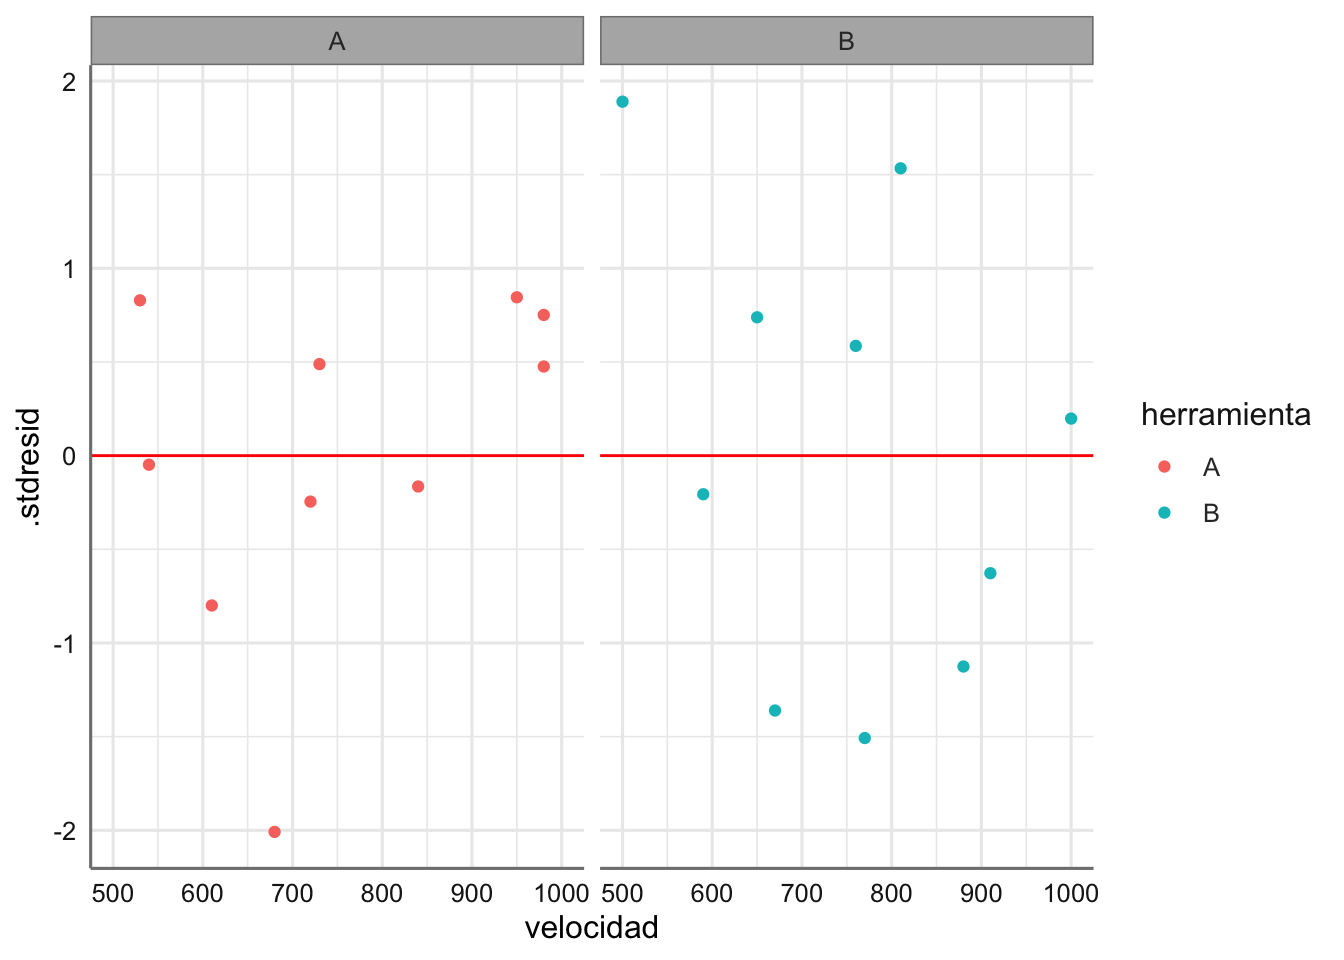
\includegraphics{libroSTAT_files/figure-latex/ancov005-1.pdf}

\begin{Shaded}
\begin{Highlighting}[]
\CommentTok{# Tests de hipótesis}
\KeywordTok{ols_test_normality}\NormalTok{(fit.vida)}
\end{Highlighting}
\end{Shaded}

\begin{verbatim}
## -----------------------------------------------
##        Test             Statistic       pvalue  
## -----------------------------------------------
## Shapiro-Wilk              0.9715         0.7858 
## Kolmogorov-Smirnov        0.1232         0.8859 
## Cramer-von Mises          1.4412          2e-04 
## Anderson-Darling          0.2652         0.6555 
## -----------------------------------------------
\end{verbatim}

\begin{Shaded}
\begin{Highlighting}[]
\KeywordTok{leveneTest}\NormalTok{(.stdresid }\OperatorTok{~}\StringTok{ }\NormalTok{herramienta, }\DataTypeTok{data =}\NormalTok{ diagnostico)}
\end{Highlighting}
\end{Shaded}

\begin{verbatim}
## Levene's Test for Homogeneity of Variance (center = median)
##       Df F value Pr(>F)
## group  1  1.3888  0.254
##       18
\end{verbatim}

\begin{Shaded}
\begin{Highlighting}[]
\CommentTok{# Análisis de influencia}
\KeywordTok{ols_plot_cooksd_chart}\NormalTok{(fit.vida)}
\end{Highlighting}
\end{Shaded}

\includegraphics{libroSTAT_files/figure-latex/ancov005-2.pdf}

Los residuos tienen un comportamiento aleatorio, se verifican las hipótesis del modelo y no se detectan observaciones influyentes. El modelo obtneido parace adecuado para estudiar el tiempo de vida en función de la velocidad y la herramienta utilizada.

\hypertarget{datos-de-longevidad-1}{%
\subsubsection{Datos de longevidad}\label{datos-de-longevidad-1}}

Obtenemos los valores de diagnóstico y realizamos los correspondientes tests de hipótesis y análisis de influencia.

\begin{Shaded}
\begin{Highlighting}[]
\CommentTok{# Valores de diagnóstico}
\NormalTok{diagnostico <-}\StringTok{ }\KeywordTok{fortify}\NormalTok{(fit.longevidad)}
\CommentTok{# Gráfico}
\KeywordTok{ggplot}\NormalTok{(diagnostico,}\KeywordTok{aes}\NormalTok{(}\DataTypeTok{x =}\NormalTok{ thorax, }\DataTypeTok{y =}\NormalTok{ .stdresid, }\DataTypeTok{colour =}\NormalTok{ actividad)) }\OperatorTok{+}\StringTok{ }
\StringTok{   }\KeywordTok{geom_point}\NormalTok{() }\OperatorTok{+}
\StringTok{   }\KeywordTok{geom_hline}\NormalTok{(}\DataTypeTok{yintercept =} \DecValTok{0}\NormalTok{, }\DataTypeTok{col =} \StringTok{"red"}\NormalTok{)}\OperatorTok{+}
\StringTok{   }\KeywordTok{facet_wrap}\NormalTok{(. }\OperatorTok{~}\StringTok{ }\NormalTok{actividad)}
\end{Highlighting}
\end{Shaded}

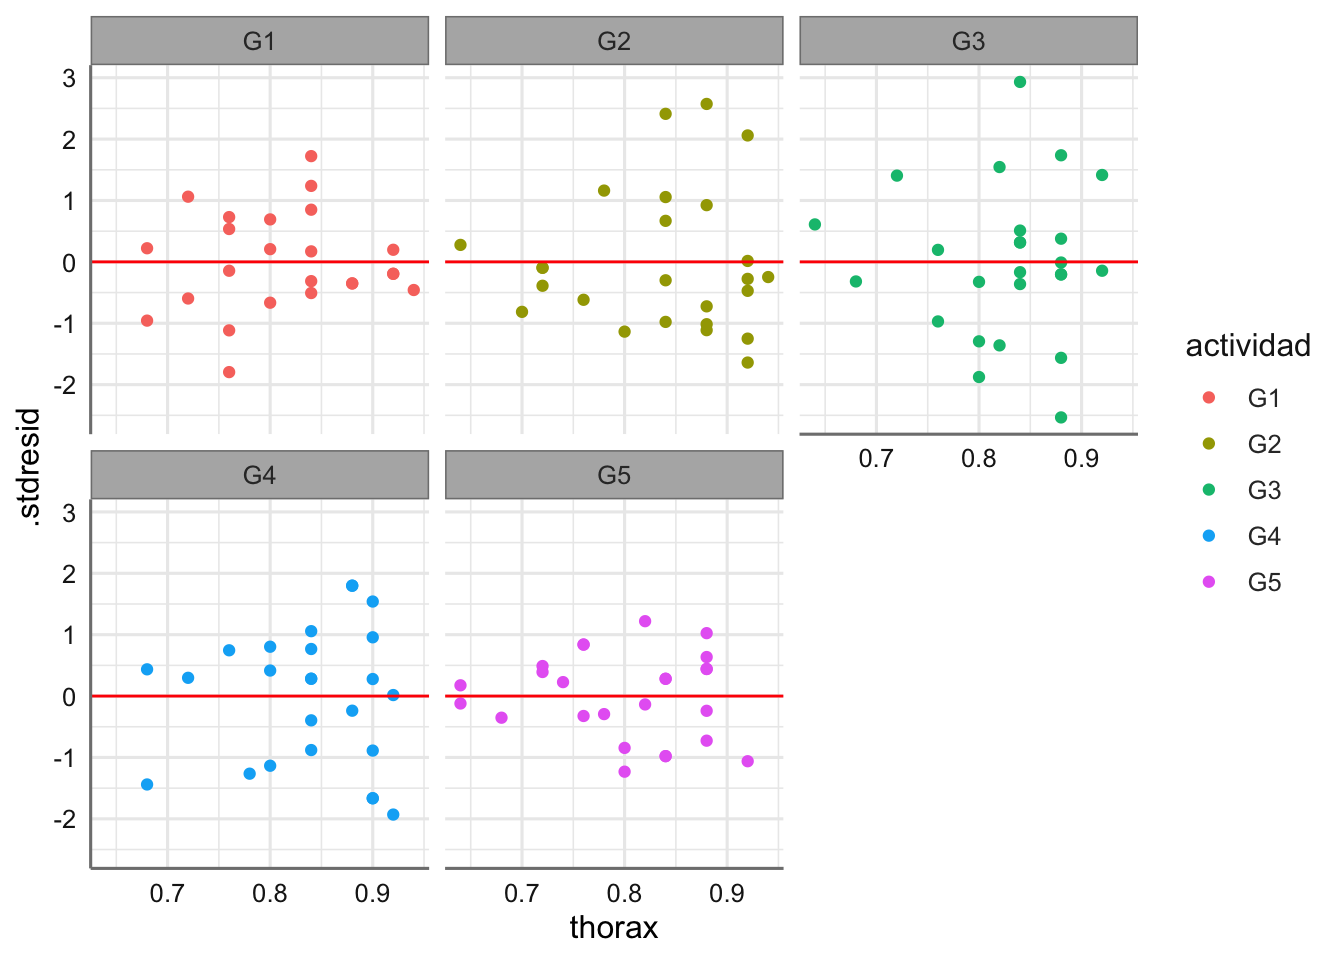
\includegraphics{libroSTAT_files/figure-latex/ancov006-1.pdf}

\begin{Shaded}
\begin{Highlighting}[]
\CommentTok{# Tests de hipótesis}
\KeywordTok{ols_test_normality}\NormalTok{(fit.longevidad)}
\end{Highlighting}
\end{Shaded}

\begin{verbatim}
## -----------------------------------------------
##        Test             Statistic       pvalue  
## -----------------------------------------------
## Shapiro-Wilk              0.9916         0.6607 
## Kolmogorov-Smirnov        0.0538         0.8654 
## Cramer-von Mises         10.2413         0.0000 
## Anderson-Darling          0.3224         0.5241 
## -----------------------------------------------
\end{verbatim}

\begin{Shaded}
\begin{Highlighting}[]
\KeywordTok{leveneTest}\NormalTok{(.stdresid }\OperatorTok{~}\StringTok{ }\NormalTok{actividad, }\DataTypeTok{data =}\NormalTok{ diagnostico)}
\end{Highlighting}
\end{Shaded}

\begin{verbatim}
## Levene's Test for Homogeneity of Variance (center = median)
##        Df F value Pr(>F)
## group   4  1.2925 0.2769
##       119
\end{verbatim}

\begin{Shaded}
\begin{Highlighting}[]
\CommentTok{# Análisis de influencia}
\KeywordTok{ols_plot_cooksd_chart}\NormalTok{(fit.longevidad)}
\end{Highlighting}
\end{Shaded}

\includegraphics{libroSTAT_files/figure-latex/ancov006-2.pdf}

Aunque se verifican las hipótesis del modelo y no se detectan observaciones influyentes, si que es cierto que los gráficos de residuos muestram cierto comportamiento de embudo con varaibilidades más pequeñas en valores más pequeños de thorax, y mayor dispersión al aumentar la longitud del thorax. Sería recomendable probar Box-Cox para tratar de obtner una transfromación de la respuesta que nos permita obteenr gráficos sin esos efectos indeseables.

\begin{Shaded}
\begin{Highlighting}[]
\NormalTok{MASS}\OperatorTok{::}\KeywordTok{boxcox}\NormalTok{(fit.longevidad)}
\end{Highlighting}
\end{Shaded}

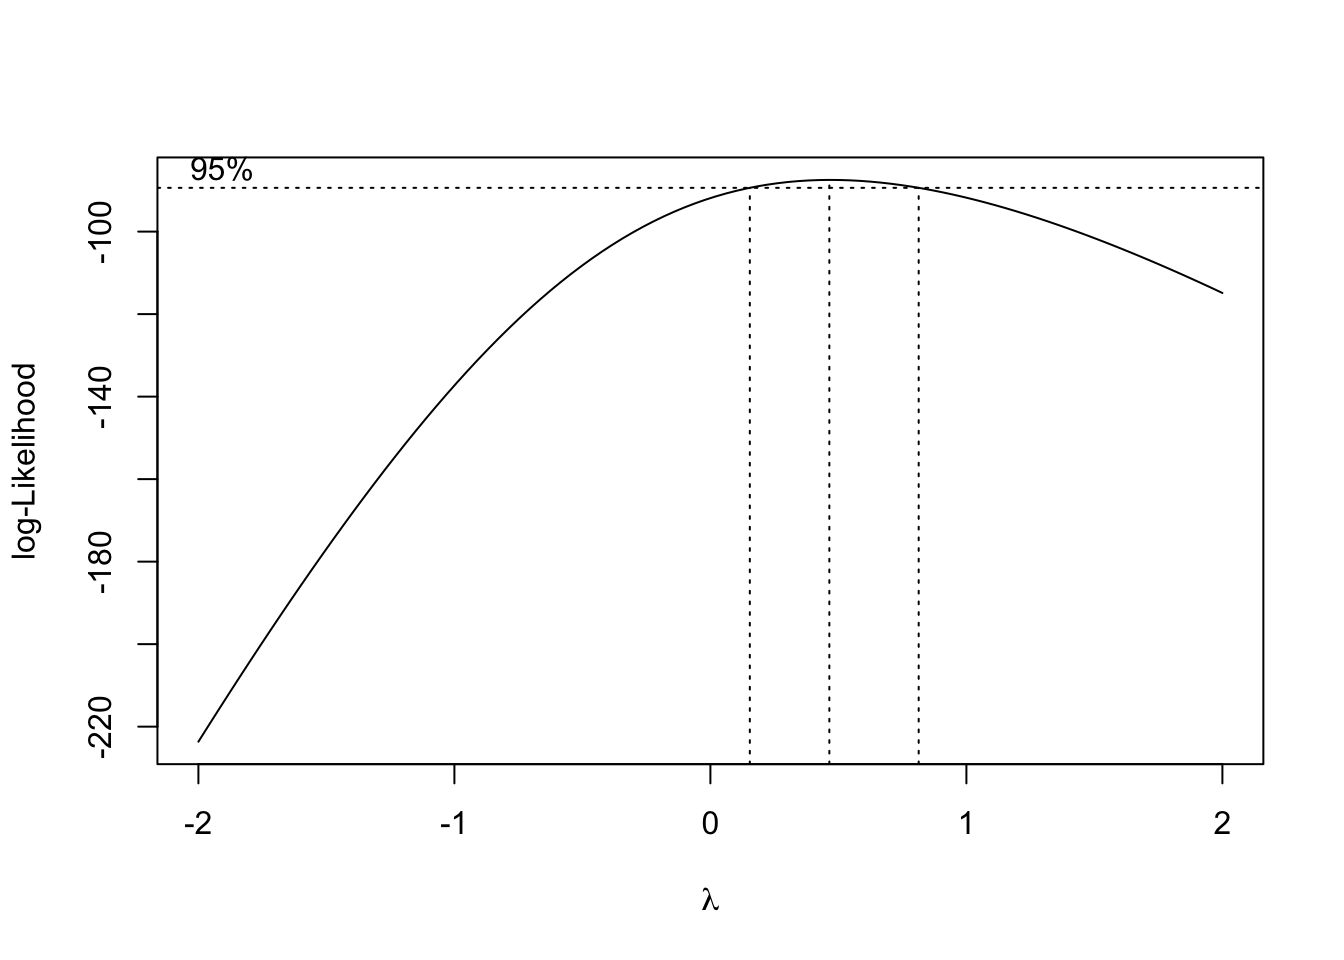
\includegraphics{libroSTAT_files/figure-latex/ancov007-1.pdf}

La transformación raíz cuadrada parece adecuada en esta situación. Obtenemos la nueva variable y ajustamos de nuevo el modelo.

\begin{Shaded}
\begin{Highlighting}[]
\CommentTok{# Trnasformación}
\NormalTok{longevidad <-}\StringTok{ }\NormalTok{longevidad }\OperatorTok\StringTok{ }\KeywordTok{mutate}\NormalTok{(}\DataTypeTok{rlongevidad =} \KeywordTok{sqrt}\NormalTok{(longevidad)) }
\CommentTok{# Modelo saturado}
\NormalTok{fit.longevidad <-}\StringTok{ }\KeywordTok{lm}\NormalTok{(rlongevidad }\OperatorTok{~}\StringTok{ }\NormalTok{thorax }\OperatorTok{*}\StringTok{ }\NormalTok{actividad, }\DataTypeTok{data =}\NormalTok{ longevidad)}
\CommentTok{# Selección del modelo}
\KeywordTok{ols_step_backward_p}\NormalTok{(fit.longevidad, }\DataTypeTok{prem =} \FloatTok{0.05}\NormalTok{)}
\end{Highlighting}
\end{Shaded}

\begin{verbatim}
## 
## 
##                                Elimination Summary                                
## ---------------------------------------------------------------------------------
##         Variable                          Adj.                                       
## Step        Removed         R-Square    R-Square     C(p)        AIC        RMSE     
## ---------------------------------------------------------------------------------
##    1    thorax:actividad      0.6868      0.6736    -3.0694    267.2943    0.6888    
## ---------------------------------------------------------------------------------
\end{verbatim}

De nuevo el modelo seleccionado prescinde del efecto de interacción. Ajustamos y estudiamos el nuevo modelo.

~

rlongevidad

Predictors

Estimates

CI

(Intercept)

0.34

-1.03~--~1.71

thorax

9.41

7.77~--~11.06

actividad {[}G2{]}

-0.30

-0.69~--~0.09

actividad {[}G3{]}

-0.12

-0.51~--~0.27

actividad {[}G4{]}

-0.76

-1.15~--~-0.37

actividad {[}G5{]}

-1.73

-2.12~--~-1.34

Observations

124

¿Cuáles son las ecuaciones de estimación en este caso?

El proceso de diagnóstico para el nuevo modelo permite verificar el cumplimineto de las hipótesis y la leve mejora de los gráficos de residuos.

\begin{Shaded}
\begin{Highlighting}[]
\CommentTok{# Valores de diagnóstico}
\NormalTok{diagnostico <-}\StringTok{ }\KeywordTok{fortify}\NormalTok{(fit.longevidad)}
\CommentTok{# Gráfico}
\KeywordTok{ggplot}\NormalTok{(diagnostico,}\KeywordTok{aes}\NormalTok{(}\DataTypeTok{x =}\NormalTok{ thorax, }\DataTypeTok{y =}\NormalTok{ .stdresid, }\DataTypeTok{colour =}\NormalTok{ actividad)) }\OperatorTok{+}\StringTok{ }
\StringTok{   }\KeywordTok{geom_point}\NormalTok{() }\OperatorTok{+}
\StringTok{   }\KeywordTok{geom_hline}\NormalTok{(}\DataTypeTok{yintercept =} \DecValTok{0}\NormalTok{, }\DataTypeTok{col =} \StringTok{"red"}\NormalTok{)}\OperatorTok{+}
\StringTok{   }\KeywordTok{facet_wrap}\NormalTok{(. }\OperatorTok{~}\StringTok{ }\NormalTok{actividad)}
\end{Highlighting}
\end{Shaded}

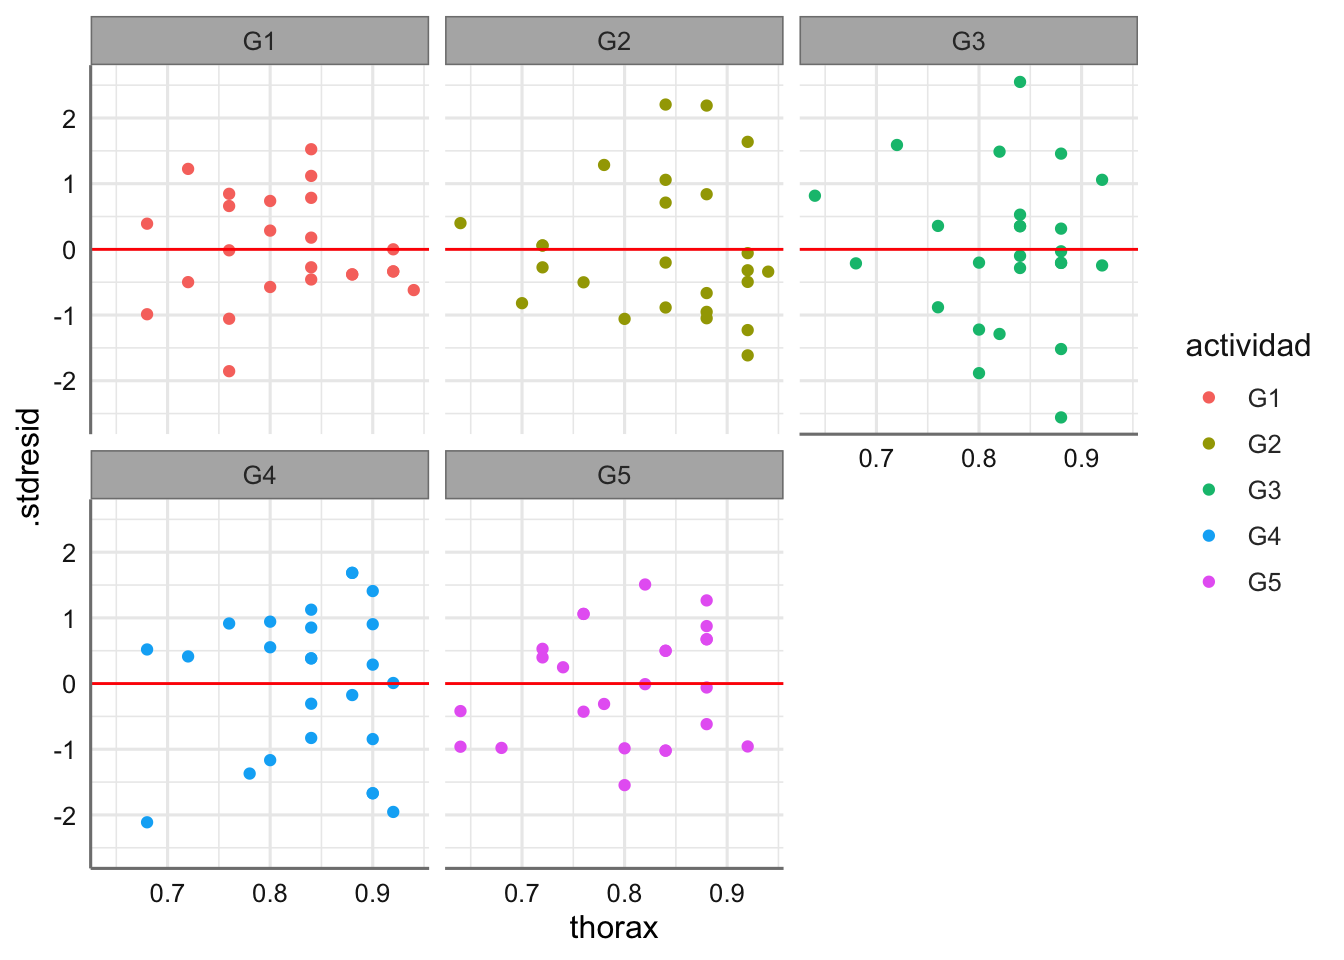
\includegraphics{libroSTAT_files/figure-latex/ancov010-1.pdf}

\begin{Shaded}
\begin{Highlighting}[]
\CommentTok{# Tests de hipótesis}
\KeywordTok{ols_test_normality}\NormalTok{(fit.longevidad)}
\end{Highlighting}
\end{Shaded}

\begin{verbatim}
## -----------------------------------------------
##        Test             Statistic       pvalue  
## -----------------------------------------------
## Shapiro-Wilk              0.9951         0.9465 
## Kolmogorov-Smirnov        0.0474         0.9432 
## Cramer-von Mises         10.7431         0.0000 
## Anderson-Darling          0.2137         0.8484 
## -----------------------------------------------
\end{verbatim}

\begin{Shaded}
\begin{Highlighting}[]
\KeywordTok{leveneTest}\NormalTok{(.stdresid }\OperatorTok{~}\StringTok{ }\NormalTok{actividad, }\DataTypeTok{data =}\NormalTok{ diagnostico)}
\end{Highlighting}
\end{Shaded}

\begin{verbatim}
## Levene's Test for Homogeneity of Variance (center = median)
##        Df F value Pr(>F)
## group   4  0.6856 0.6033
##       119
\end{verbatim}

\begin{Shaded}
\begin{Highlighting}[]
\CommentTok{# Análisis de influencia}
\KeywordTok{ols_plot_cooksd_chart}\NormalTok{(fit.longevidad)}
\end{Highlighting}
\end{Shaded}

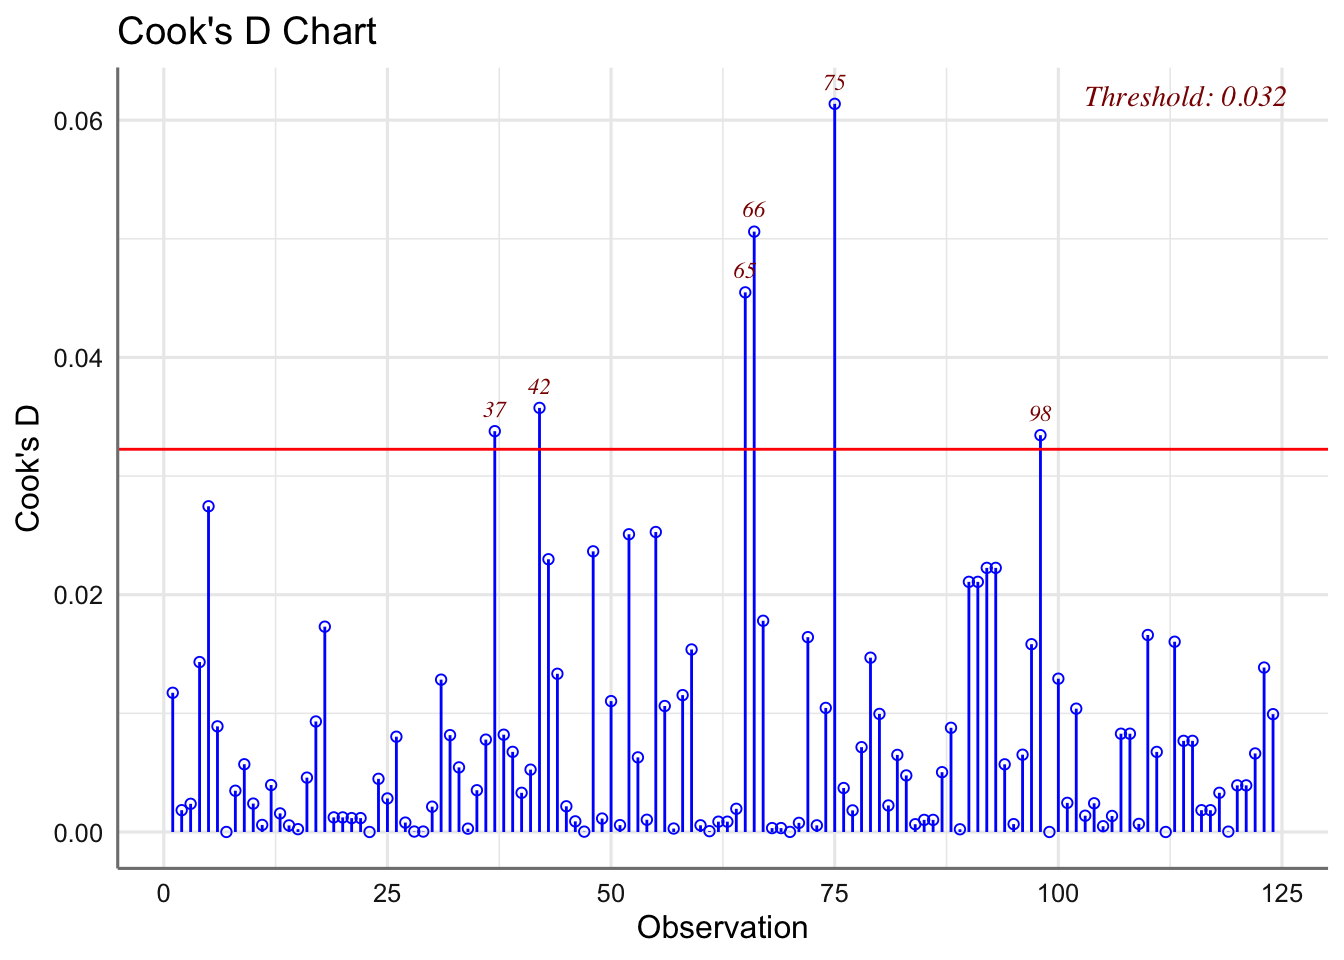
\includegraphics{libroSTAT_files/figure-latex/ancov010-2.pdf}

\hypertarget{predicciuxf3n}{%
\section{Predicción}\label{predicciuxf3n}}

El proceso de predicción en este tipo de modelos es muy simple a partir de las ecuaciones de los modelos obtenidas. De hecho, en las secciones anteriores ya hemos visto gráficamente la predicción para todos estos modelos en los ejemplos que hemos ido trabajando. Básicamente, si queremos obtener una predicción especifica deberemos dar un valor del factor y otro de la predictora numérica para calcular el valor de predicción y su correspondiente intervalo. En este caso nos imitamos a representar las bandas de predicción que podemos obtener para cada modelo.

\hypertarget{ejemplos-2}{%
\subsection{Ejemplos}\label{ejemplos-2}}

Construimos la predicción y bandas de confianza para cada uno de los ejemplos a aprtir de los modelos determinados tras la fase de diagnóstico.

\hypertarget{datos-de-tiempo-de-vida-2}{%
\subsubsection{Datos de tiempo de vida}\label{datos-de-tiempo-de-vida-2}}

A continuación se presentan las rectas de predicción para el modelo ajustado a este abnco de datos.

\begin{Shaded}
\begin{Highlighting}[]
\KeywordTok{plot_model}\NormalTok{(fit.vida, }\StringTok{"pred"}\NormalTok{, }\DataTypeTok{terms =} \KeywordTok{c}\NormalTok{(}\StringTok{"velocidad"}\NormalTok{,}\StringTok{"herramienta"}\NormalTok{),}
           \DataTypeTok{title =}\StringTok{"Predicción de la media del tiempo de vida"}\NormalTok{)}
\end{Highlighting}
\end{Shaded}

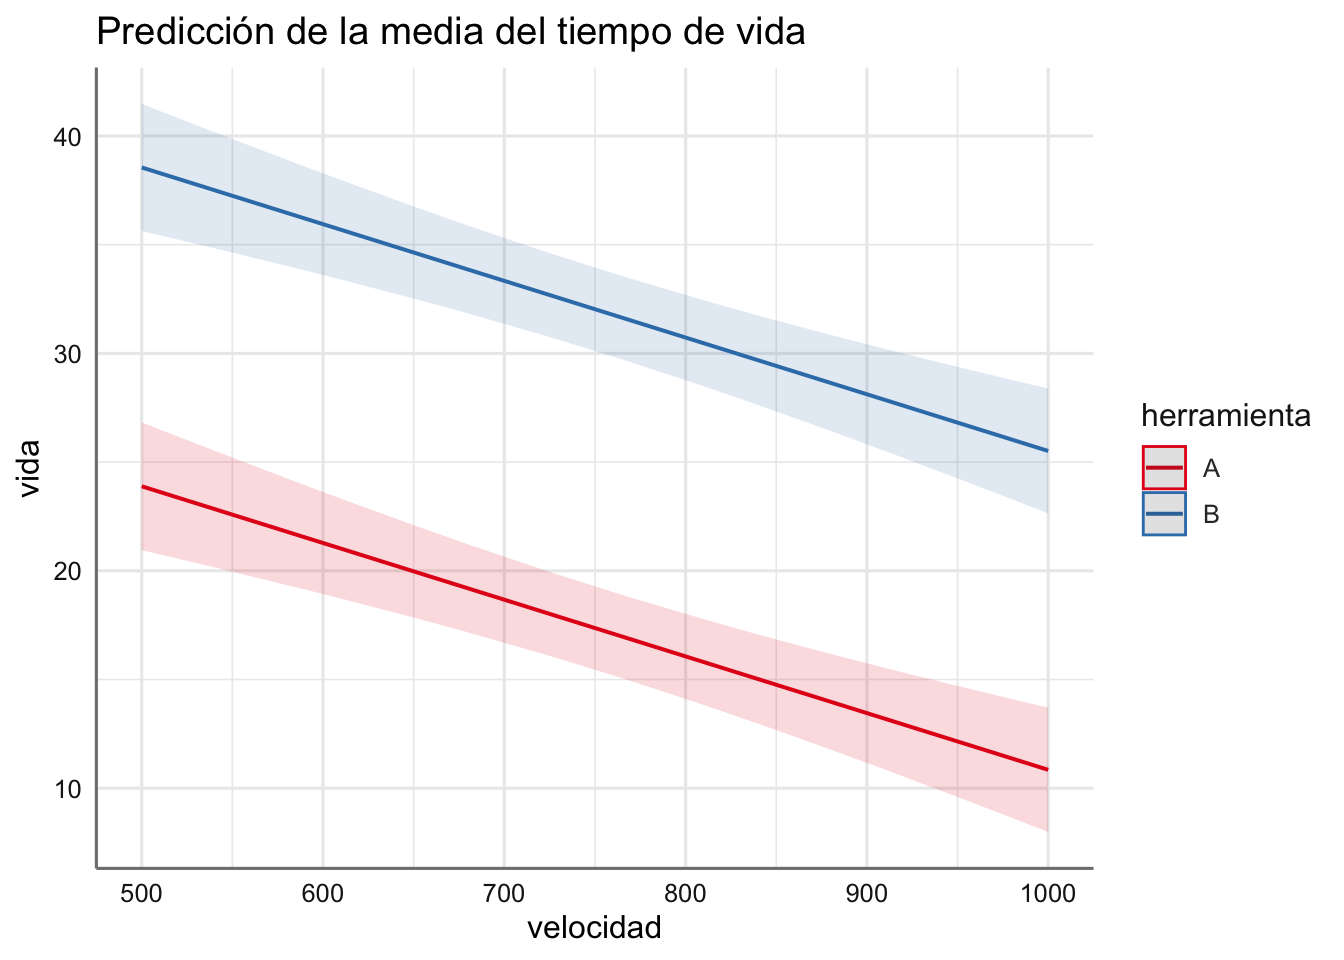
\includegraphics{libroSTAT_files/figure-latex/ancov011-1.pdf}

\hypertarget{datos-de-longevidad-2}{%
\subsubsection{Datos de longevidad}\label{datos-de-longevidad-2}}

A continuación se presentan las rectas de predicción para el modelo ajustado a este abnco de datos.

\begin{Shaded}
\begin{Highlighting}[]
\KeywordTok{plot_model}\NormalTok{(fit.longevidad, }\StringTok{"pred"}\NormalTok{, }\DataTypeTok{terms =} \KeywordTok{c}\NormalTok{(}\StringTok{"thorax"}\NormalTok{,}\StringTok{"actividad"}\NormalTok{),}
           \DataTypeTok{title =}\StringTok{"Predicción de la raíz cuadrada de la media de longevidad"}\NormalTok{)}
\end{Highlighting}
\end{Shaded}

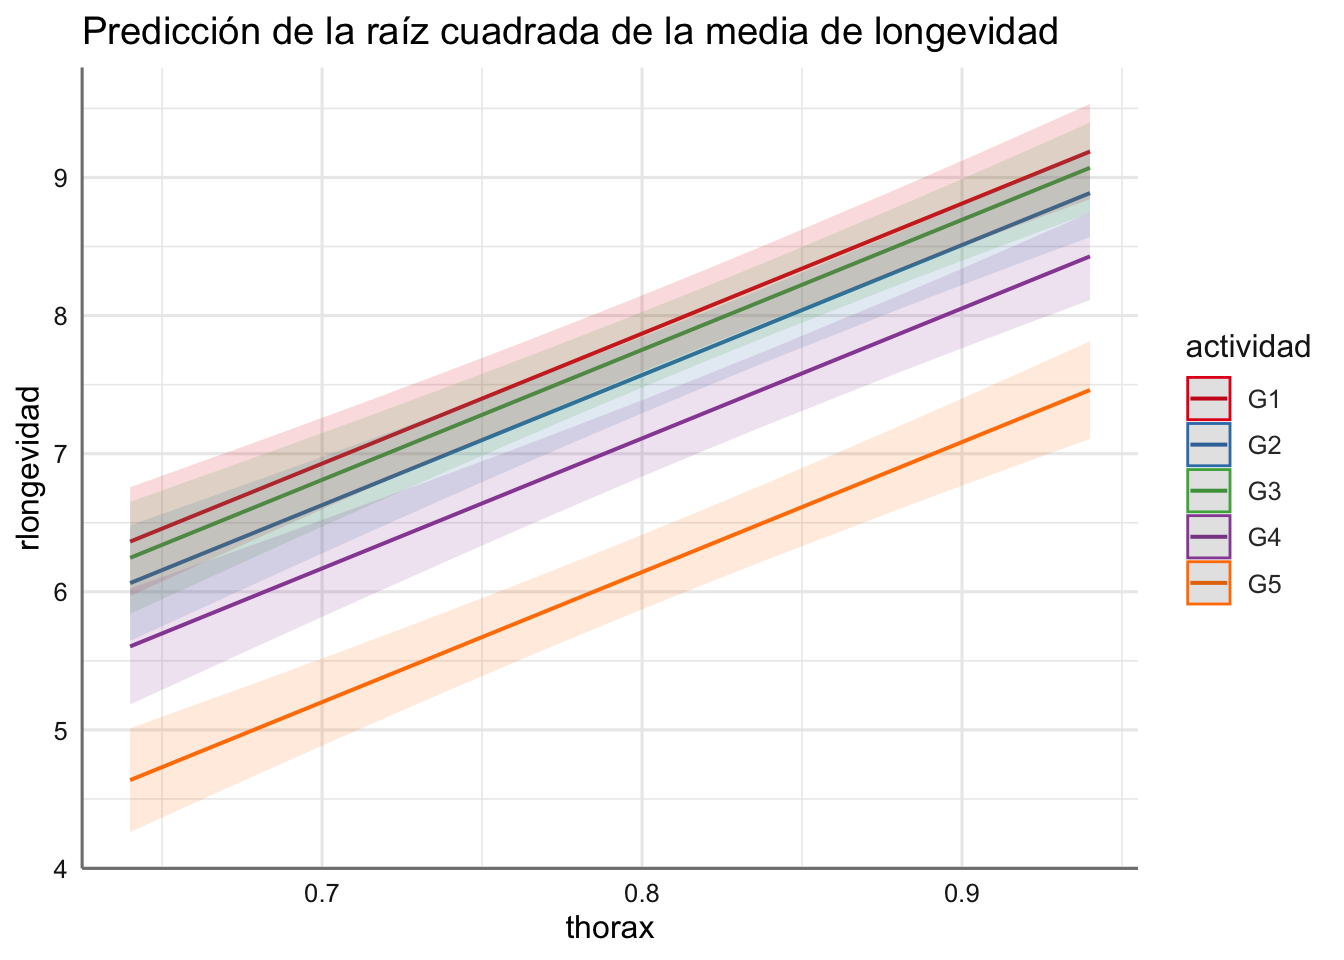
\includegraphics{libroSTAT_files/figure-latex/ancov012-1.pdf}

\hypertarget{ejercicios}{%
\section{Ejercicios}\label{ejercicios}}

A continuación se presenta la colección de ejercicios de esta unidad.

\textbf{Ejercicio 1.} Disponemos de los datos de peso de 24 niños recién nacidos (\texttt{peso}), su sexo (\texttt{sexo}; ``H'' = Hombres y ``M'' = Mujeres) y la edad de sus madres (\texttt{edad}). Nos gustaría ser capaces de determinar un modelo que explique el peso de los niños recién nacidos en función de su sexo y de la edad de sus madres.

\begin{Shaded}
\begin{Highlighting}[]
\CommentTok{# Lectura de datos}
\NormalTok{edad <-}\StringTok{ }\KeywordTok{c}\NormalTok{(}\DecValTok{40}\NormalTok{, }\DecValTok{38}\NormalTok{, }\DecValTok{40}\NormalTok{, }\DecValTok{35}\NormalTok{, }\DecValTok{36}\NormalTok{, }\DecValTok{37}\NormalTok{, }\DecValTok{41}\NormalTok{, }\DecValTok{40}\NormalTok{, }\DecValTok{37}\NormalTok{, }\DecValTok{38}\NormalTok{, }\DecValTok{40}\NormalTok{, }\DecValTok{38}\NormalTok{,}
          \DecValTok{40}\NormalTok{, }\DecValTok{36}\NormalTok{, }\DecValTok{40}\NormalTok{, }\DecValTok{38}\NormalTok{, }\DecValTok{42}\NormalTok{, }\DecValTok{39}\NormalTok{, }\DecValTok{40}\NormalTok{, }\DecValTok{37}\NormalTok{, }\DecValTok{36}\NormalTok{, }\DecValTok{38}\NormalTok{, }\DecValTok{39}\NormalTok{, }\DecValTok{40}\NormalTok{)}
\NormalTok{peso <-}\StringTok{ }\KeywordTok{c}\NormalTok{(}\DecValTok{2968}\NormalTok{, }\DecValTok{2795}\NormalTok{, }\DecValTok{3163}\NormalTok{, }\DecValTok{2925}\NormalTok{, }\DecValTok{2625}\NormalTok{, }\DecValTok{2847}\NormalTok{, }\DecValTok{3292}\NormalTok{, }\DecValTok{3473}\NormalTok{, }\DecValTok{2628}\NormalTok{, }\DecValTok{3176}\NormalTok{,}
          \DecValTok{3421}\NormalTok{, }\DecValTok{2975}\NormalTok{, }\DecValTok{3317}\NormalTok{, }\DecValTok{2729}\NormalTok{, }\DecValTok{2935}\NormalTok{, }\DecValTok{2754}\NormalTok{, }\DecValTok{3210}\NormalTok{, }\DecValTok{2817}\NormalTok{, }\DecValTok{3126}\NormalTok{, }\DecValTok{2539}\NormalTok{,}
          \DecValTok{2412}\NormalTok{, }\DecValTok{2991}\NormalTok{, }\DecValTok{2875}\NormalTok{, }\DecValTok{3231}\NormalTok{)}
\NormalTok{sexo <-}\StringTok{ }\KeywordTok{gl}\NormalTok{(}\DecValTok{2}\NormalTok{,}\DecValTok{12}\NormalTok{, }\DataTypeTok{labels=}\KeywordTok{c}\NormalTok{(}\StringTok{"H"}\NormalTok{,}\StringTok{"M"}\NormalTok{))}
\NormalTok{ejer01 <-}\StringTok{ }\KeywordTok{data.frame}\NormalTok{(edad, peso, sexo)}
\end{Highlighting}
\end{Shaded}

\textbf{Ejercicio 2.} Se lleva a cabo una investigación sobre diversas malformaciones del sistema nervioso central registradas en nacidos vivos en Gales del Sur, Reino Unido. El estudio fue diseñado para determinar el efecto de la dureza del agua sobre la incidencia de tales malformaciones. La información registrada son: \texttt{NoCNS} = recuento de nacimientos sin problema CNS; \texttt{An} = conteo de nacimientos de Anencephalus; \texttt{Sp} = conteo de nacimientos de espina bífida; \texttt{Otro} = recuento de otros nacimientos del SNC; \texttt{Agua} = endurecimiento del agua; \texttt{Trabajo} = un factor con niveles Manual no manual en función del tipo de trabajo realizado por los padres Se está interesado en predecir el número total de malformaciones en función de la calidad del agua y el trabajo realizado por los padres.

\begin{Shaded}
\begin{Highlighting}[]
\CommentTok{# Lectura de datos}
\NormalTok{previo <-}\StringTok{ }\KeywordTok{read_csv}\NormalTok{(}\StringTok{"https://goo.gl/bNOSxt"}\NormalTok{, }\DataTypeTok{col_types =} \StringTok{"cdddddc"}\NormalTok{)}
\CommentTok{# Calculamos el número total de malformaciones}
\NormalTok{ejer02 <-}\StringTok{ }\NormalTok{previo }\OperatorTok\StringTok{ }\KeywordTok{mutate}\NormalTok{(}\DataTypeTok{CNS=}\NormalTok{An}\OperatorTok{+}\NormalTok{Sp}\OperatorTok{+}\NormalTok{Other)}
\end{Highlighting}
\end{Shaded}

\textbf{Ejercicio 3.} Se ha realizado un estudio para establecer la calidad de los vinos de la variedad Pino Noir en función de un conjunto de características analizadas. Las características analizadas son \texttt{claridad}, \texttt{aroma}, \texttt{cuerpo}, \texttt{olor} y \texttt{matiz}. Para medir la \texttt{calidad} se organiza una cata ciega a un conjunto de expertos y se calcula la puntuación final de cada vino a partir de la información de todos ellos. Además se registra la región (\texttt{region}) de procedencia del vino por si puede influir en la calidad del vino.

\begin{Shaded}
\begin{Highlighting}[]
\CommentTok{# Lectura de datos}
\NormalTok{ejer03 <-}\StringTok{ }\KeywordTok{read_csv}\NormalTok{(}\StringTok{"https://goo.gl/OX9wgM"}\NormalTok{, }\DataTypeTok{col_types =} \StringTok{"ddddddc"}\NormalTok{)}
\end{Highlighting}
\end{Shaded}

\textbf{Ejercicio 4.} Un fabricante de ropa que suministra uniformes militares debe cortar chaquetas, camisas, pantalones (variable \texttt{Prenda}) y otros complementos (en muchas tallas diferentes), de rollos de tela. La tela es cara, de modo que el desperdicio (\texttt{Desperdicio}) tiene un efecto muy grande en los beneficios. El fabricante tiene que elegir entre tres máquinas (\texttt{Maquina}) cortadoras asistidas por computadora: A, B y C. El fabricante decide experimentar haciendo que cada máquina corte varios lotes de chaquetas, varios más de camisas otros más de pantalones y complementos para determinar que máquina es más eficiente en cada caso, es decir, tratamos de conocer el desperdicio que se producirá para cada prenda y máquina.

\begin{Shaded}
\begin{Highlighting}[]
\CommentTok{# Lectura de datos}
\NormalTok{ejer04 <-}\StringTok{ }\KeywordTok{read_csv}\NormalTok{(}\StringTok{"https://bit.ly/2GcVn3R"}\NormalTok{, }\DataTypeTok{col_types =} \StringTok{"ccd"}\NormalTok{)}
\NormalTok{ejer04 <-}\StringTok{ }\NormalTok{ejer04 }\OperatorTok\StringTok{ }
\StringTok{  }\KeywordTok{mutate_if}\NormalTok{(}\KeywordTok{sapply}\NormalTok{(ejer04,is.character),as.factor)}
\end{Highlighting}
\end{Shaded}

\textbf{Ejercicio 5.} Una empresa dedicada a la fabricación de aislantes térmicos y acústicos establece un experimento que mide la pérdida de calor (\texttt{Calor}) a través de cuatro tipos diferentes de cristal para ventanas (\texttt{Cristal}) utilizando cinco graduaciones diferentes de temperatura exterior (\texttt{TempExt}). Se prueban tres hojas de cristal en cada graduación de temperatura, y se registra la pérdida de calor para cada hoja.

\begin{Shaded}
\begin{Highlighting}[]
\CommentTok{# Lectura de datos}
\NormalTok{ejer05 <-}\StringTok{ }\KeywordTok{read_csv}\NormalTok{(}\StringTok{"https://goo.gl/V6hyVW"}\NormalTok{, }\DataTypeTok{col_types =} \StringTok{"ddc"}\NormalTok{) }
\NormalTok{ejer05 <-}\StringTok{ }\NormalTok{ejer05 }\OperatorTok
\StringTok{  }\KeywordTok{mutate_if}\NormalTok{(}\KeywordTok{sapply}\NormalTok{(ejer05,is.character),as.factor) }
\end{Highlighting}
\end{Shaded}

\textbf{Ejercicio 6.} El grupo de asesores LearnStatistics ha realizado un estudio para comprobar si las empresas destinan parte de los beneficios de sus ventas en la formación de sus empleados para mejorar su competitividad. Para ellos se recoge la información sobre ventas (\texttt{Ventas}) en miles de euros, capital invertido en formación (\texttt{Capital}) en miles de euros, y el nivel de productividad de la empresa establecido por un asesor externo (\texttt{Productividad}).

\begin{Shaded}
\begin{Highlighting}[]
\CommentTok{# Lectura de datos}
\NormalTok{ejer06 <-}\StringTok{ }\KeywordTok{read_csv}\NormalTok{(}\StringTok{"https://bit.ly/2rCATaO"}\NormalTok{, }\DataTypeTok{col_types =} \StringTok{"dcd"}\NormalTok{)}
\NormalTok{ejer06 <-}\StringTok{ }\NormalTok{ejer06 }\OperatorTok\StringTok{  }
\StringTok{  }\KeywordTok{mutate_if}\NormalTok{(}\KeywordTok{sapply}\NormalTok{(ejer06,is.character),as.factor) }
\end{Highlighting}
\end{Shaded}

\textbf{Ejercicio 7.} Una empresa recibe cargamentos de material para procesar en sus almacenes (\texttt{almacen}). El objetivo básico del estudio es determinar el tiempo de procesado (\texttt{tiempo}) de los cargamentos recibidos como función del tamaño del cargamento (\texttt{tamanyo}).

\begin{Shaded}
\begin{Highlighting}[]
\CommentTok{# Lectura de datos}
\NormalTok{lectura <-}\StringTok{ }\KeywordTok{read.table}\NormalTok{(}\StringTok{"https://goo.gl/kuMNpD"}\NormalTok{, }\DataTypeTok{header =} \OtherTok{TRUE}\NormalTok{) }
\NormalTok{ejer07 <-}\StringTok{ }\KeywordTok{as_tibble}\NormalTok{(lectura) }
\end{Highlighting}
\end{Shaded}

\textbf{Ejercicio 8.} La lista Forbes500 la componen las 500 empresas con mayores ventas mundiales. En este caso se desea realizar un estudio de un grupo de empresas de la lista Forbes para intentar relacionar las \texttt{Ventas} (en millones de dólares) con los \texttt{Activos} de la empresa (en millones de dólares), el \texttt{ValorBursatil} (en millones de dólares), el número de \texttt{Empleados} (en miles de personas) y el \texttt{Sector} económico al que pertenece la empresa (Alta Tecnología, Energía, Finanzas, Manufacturas, Medico, Transportes, Venta al detalle, y Otros). Como en todos los problemas económicos resulta mucho más cómodo trabajar con las variables transformadas con el logaritmo. La variable \texttt{Empresa} es un identificador y no debe ser utilizada en el proceso de modelización.

\begin{Shaded}
\begin{Highlighting}[]
\CommentTok{# Lectura de datos}
\NormalTok{lectura <-}\StringTok{ }\KeywordTok{read.table}\NormalTok{(}\StringTok{"https://goo.gl/PHQXaW"}\NormalTok{, }\DataTypeTok{header =} \OtherTok{TRUE}\NormalTok{) }
\NormalTok{ejer08 <-}\StringTok{ }\KeywordTok{as_tibble}\NormalTok{(lectura) }
\end{Highlighting}
\end{Shaded}

\textbf{Ejercicio 9.} Se conoce como infiltración al proceso por el cual el agua (riego o lluvia) se va introduciendo bajo la superficie de un terreno cultivado. Este proceso es vital para determinar las cantidades de agua de riego necesarias, para mantener el terreno en condiciones óptimas. Un parámetro habitual que sirve para estudiar dicho proceso es la carga hidráulica (\texttt{cargahid}). Este depende tanto de la profundidad de la infiltración (\texttt{profundidad}) como del procedimiento de riego usado. Se diseña un experimento para estudiar la carga hidráulica de un terreno bajo diferentes condiciones de riego (\texttt{trata}). los resultados obtenidos aparecen en la base de datos correspondiente.

\begin{Shaded}
\begin{Highlighting}[]
\CommentTok{# Lectura de datos}
\NormalTok{lectura <-}\StringTok{ }\KeywordTok{read.table}\NormalTok{(}\StringTok{"https://goo.gl/1JnUVX"}\NormalTok{, }\DataTypeTok{header =} \OtherTok{TRUE}\NormalTok{) }
\NormalTok{ejer09 <-}\StringTok{ }\KeywordTok{as_tibble}\NormalTok{(lectura)}
\end{Highlighting}
\end{Shaded}

\backmatter
  \bibliography{book.bib,packages.bib}

\end{document}
